\documentclass[a4paper, 12pt]{report}

\usepackage{graphicx}
\usepackage{float}
\usepackage{tgcursor}
\usepackage{wrapfig}
\usepackage[font=small,labelfont=bf]{caption}
\usepackage{index}
\usepackage{hyperref}
\hypersetup{
    colorlinks=true,
    linkcolor=black,
    filecolor=magenta,
    urlcolor=blue,
    }
\usepackage{amsmath}
\usepackage{xcolor}
\usepackage{listings}
\usepackage{ragged2e}
\usepackage{fancyhdr}
\usepackage{geometry}
\usepackage{zref-perpage}
\zmakeperpage{footnote}
\usepackage{xepersian}

\captionsetup[figure]{font=small}

\makeatletter
\renewcommand\@endpart{\vfil
              \if@twoside
                \null
                \thispagestyle{empty}%
                \newpage
              \fi
              \if@tempswa
                \twocolumn
              \fi}
\makeatother

\renewcommand{\baselinestretch}{1.6}

\newcommand{\lrbold}[1]{\lr{\textbf{#1}}}
\newcommand{\lrboldit}[1]{\lr{\textit{#1}}}
\newcommand{\lrit}[1]{\lr{\textit{#1}}}



\settextfont{B Zar}
\setlatintextfont[Scale=1]{Times New Roman}
\DefaultMathsDigits

% -- define code style

\definecolor{customblue}{RGB}{246, 247, 246}
\definecolor{keywordcolor}{RGB}{157, 0, 236}
\definecolor{codepurple}{rgb}{0.58,0,0.82}
\definecolor{stringcolor}{RGB}{0, 130, 0}
\definecolor{light-gray}{gray}{0.95}
\lstdefinestyle{C++Style}{%
  backgroundcolor=\color{customblue},
  breaklines=true,
  basicstyle=\footnotesize\ttfamily,
  keywordstyle=\color{keywordcolor},
  commentstyle=\color{stringcolor}\textit,
  stringstyle=\color{codepurple},
  numbers=left,
  numberstyle={\tiny\lr},
  showspaces = false,
  showstringspaces = false,
  tabsize = 4,
  frame=single,
  xleftmargin=0pt,
  xrightmargin=0pt,
  language =  C++,
  aboveskip = 20pt,
  rulecolor=\color{customblue},
  captiondirection=RTL,
}


\lstnewenvironment{C++Code}[1][]
{%
    \lstset{style=C++Style, #1}%
}{}
\newfontfamily\myfont{Nazanin Bold}
\newfontfamily\titrfont{B Titr}
\newfontfamily\mitrafont{Mitra}
\newfontfamily\zarfont{B Zar}
\newfontfamily\zarbold{Zar}

% end code style defenition

%\title{ مقدمه ای بر گرافیک کامپیوتر}
%\author{احمد منصوری و \lr{\textsf{\textbf{peter shirley}}}}
%\date{\lr{December 21, 2009}}

\pagestyle{fancy}
\fancyhf{}
\renewcommand{\headrulewidth}{0pt}
\cfoot{\thepage}


\geometry{right=4cm, left=2.5cm, top=4cm, bottom=2.5cm}

\begin{document}
%\maketitle
\let\cleardoublepage\clearpage
% title page ---------------------

\justifying
\thispagestyle{empty}
\mbox{}
\newpage
\thispagestyle{empty}
  \vfill
  \begin{center}
      
\includegraphics [width=9cm] {images/page2.jpg}
  \end{center}
  \vfill

\begin{titlepage}
\begin{figure}[H]
    \centering
        
\includegraphics[width=8cm]{images/logo.png}
\end{figure}

% \vspace*{1cm}
    \begin{center}
      \large
      {\fontsize{13}{1cm} \selectfont \myfont \textbf{دانشگاه شهید باهنر کرمان}\par}
      {\fontsize{12}{1cm} \selectfont \myfont \textbf{دانشکده فنی و مهندسی}\par}
      {\fontsize{18}{1cm} \selectfont \myfont \textbf{پروژه کارشناسی رشته مهندسی کامپیوتر}\par}
      {\fontsize{18}{1cm} \selectfont \titrfont \textbf{عنوان}:
      \titrfont \textbf{پیاده سازی \lr{Real-time Render Engine}}\par}
      {\fontsize{15}{1cm} \selectfont \myfont \textbf{استاد راهنما: سرکار خانم دکتر قاسمیان}\par}
      {\fontsize{15}{1cm} \selectfont \myfont \textbf{دانشجو: احمد منصوری بیدخوانی}\par}
      \normalsize
      {\fontsize{13}{1cm} \selectfont \myfont \textbf{تابستان 1400}}
    \end{center}

\end{titlepage}


% end title page -----------------
\fontsize{13}{1cm}\mitrafont\textbf{چکیده}
\normalsize
\begin{flushright}
\justifying
\fontsize{13}{0.8cm}\mitrafont
  همزمان با پیدایش کامپیوتر ها، تلاش ها برای بهره بردن از توان آنها برای ساخت ابزار های تصویر کردن\footnote{\lr{visualize}} داده ها و ابزار های مربوطه برای
  استفاده از قدرت کامپیوتر در زمینه های نظامی، فیلم و انیمیشن، شبیه سازی و بازی سازی شروع شد.\par
    طراحی و پیاده سازی موتور های رندر سه بعدی\footnote{\lr{3D render engine}} به صورت کلی دارای پایه ها و دانشی یکسان از نحوه کار پردازنده ها و ریاضیات است.\par
    هدف این پروژه مطالعه و ساخت یک  موتور رندر سه بعدی بی درنگ\footnote{\lr{real-time render engine}} و بررسی تکنیک ها و روش های جایگزین برای استفاده در صنایع و پروژه های مختلف است. \lr{render engine} ها پایه های اصلی تمامی شبیه ساز ها، ابزار های صنعتی، بازی های کامپیوتری و ابزارآلات مربوط به صنعت فیلم و انیمیشن می باشند که در دسته بندی های مختلفی ساخته می شوند، این پروژه مربوط به ساختن دسته بندی خاصی از این موتور ها یعنی دسته بندی \lr{real time} می شود که کاربرد زیادی در تمامی زمینه های بالا به خصوص صنعت بازی های رایانه ای دارد.
   در انتهای این گزارش فصلی برای نمایش برخی از قابلیت های یک \lr{realtime render engine} اختصاص داده شده.

\end{flushright}


\begingroup
  \hypersetup{hidelinks}
  \tableofcontents
  \listoffigures
\endgroup

\makeatletter
\renewcommand\@endpart{\vfil
              \if@twoside
                \null
                \thispagestyle{empty}%
                \newpage
              \fi
              \if@tempswa
                \twocolumn
              \fi}
\makeatother

\chapter{\fontsize{18pt}{1.0cm}\zarbold\lrbold{Renderer}}


\fontsize{13pt}{1cm}\zarfont
% \part{گرافیک}

\huge
    مقدمه

% \vspace*{2cm}
\normalsize
    \lr{real time rendering} به تولید متناوب تصاویر بر مبنای تغییرات مدل ها یا دوربین در فضای نرم افزار گفته می شود. ابزار دستیابی به این هدف \lr{real-time rendering engine} ها هستند.\par
    هدف این پروژه مطالعه ساختار ها و تکنیک ها در این زمینه و پیاده سازی آن ها به منظور دستیابی به این توانایی است.\par
    تاریحچه استفاده از گرافیک کامپیوتری\footnote{\lr{Computer Graphics}} به دهه پنجاه قرن بیستم میلادی در عرصه جنگ سرد و بعدتر در زمینه رصد کردن تصویری رادار ها برمی گردد، در دهه شصت، استفاده از این تکنولوژی در زمینه بازی های ویدیوئی\footnote{\lr{video games}} منجر به تولید یکی از مهم ترین بازی های ویدیویی یعنی \lr{spacewar} انجامید و سبب علاقمندی به این نوع سرگرمی شد، دهه هفتاد و با اوج گیری پیشرفت های سخت افزاری، پیشرفت های چشمگیری در زمینه گرافیک کامپیوتر به وجود آمد که این روند تا سال های اخیر و با معرفی کارت گرافیک هایی با قابلیت استفاده بی درنگ از الگوریتم های دنبال کردن مسیر نور \footnote{\lr{RTX (real-time ray tracing)}} ادامه داشته است.\par
    ترتیب نگارش بخش های مختلف پایان نامه بر اساس مراحل ساخت یک \lr{real-time render engine} خواهد بود.
\newpage

%\addcontentsline{toc}{section}{پنجره ها و کانتکست ها}
\section{\fontsize{15pt}{1.0cm}\zarbold\textbf{پنجره ها و کانتکست ها}}
\vspace*{0.6cm}

\subsection{\lr{openGL}}
\normalsize
    \lrboldit{OpenGL} یک \lrboldit{api}  چند زبانه\footnote{\lr{Cross Language}} و چند سکویی \footnote{\lr{Cross Platform}} است که برای به تصویر کشیدن تصاویر دو بعدی و سه بعدی با استفاده از بردار ها\footnote{\lr{vectors}}
    اسفاده می شود، معمولا از \lrboldit{OpenGL} برای برقراری ارتباط با واحد پردازش گرافیکی \lrboldit{(GPU)} و بهره بردن از سرعت سخت افزار مخصوص برای رندر استفاده می شود.\par

    همچنین \lrit{api} های دیگری نیز برای استفاده از قدرت سخت افزاری و پردازنده گرافیکی وجود دارند، \lrit{Vulkan} نیز مانند \lrit{openGL} چند زبانی و چند سکویی است،
    \lrit{DirectX} به صورت انحصاری توسط مایکروسافت توسعه می یابد و در سیستم عامل ویندوز استفاده می شود ، شرکت \lr{Apple} از \lrit{api} اختصاصی خود به نام \lrit{Metal}
    به صورت انحصاری پشتیبانی می کند، دلیل انتخاب\lrit{openGL} در این پروژه چندسکویی بودن و ساختار ساده تر برای پروژه های آموزشی در زمینه \lr{real-time rendering} می باشد.\par

    نباید \lrit{OpenGL} را با یک کتابخانه\footnote{\lr{library}} اشتباه گرفت، \lrbold{OpenGL} به صورت یک \lr{interface} و یک قراداد انتزاعی در ورژن های مختلف ارائه می شود که فروشندگان و سازندگان\lrit{(vendor)} مختلف باید پیاده سازی ای منطبق با این قرارداد را انجام دهند.
    پس از نصب درایور مربوط به پردازنده گرافیکی، برنامه نویس قابلیت دسترسی به تابع های مختلف که توسط \lrit{vendor} پیاده سازی شده را خواهد داشت.
    برای استفاده از \lrit{{OpenGL}} نیاز به ابزار های دیگری نیز داریم، ابتدا نیاز داریم که یک \lrit{window} و یک \lrit{context} تعریف کنیم،
    برای این کار از \lrbold{GLFW} استفاده می کنیم.


\newpage
\subsection{\lr{GLFW}}
\noindent
\normalsize
    یک کتابخانه برای ساختن \lrit{window} و \lrit{context} ها برای \lrit{openGL, openGL ES, Vulkan} است، این کتابخانه به زبان \lrbold{C} نوشته شده و \lrit{binding} های مختلف آن به زبان های مختلف موجود است، این کتابخانه همچنین توانایی کنترل کردن ورودی های مختلف مثل \lrit{keyboard, mouse, joystick} را داراست، ما برای استفاده از \lrit{openGL} نیاز به این کتابخانه یا مشابه آن داریم زیرا \lr{openGL} هیچگونه قابلیت پیشفرضی برای مدیریت \lr{window} یا \lr{context} ها یا مدیریت \lr{input} ندارد. همچنین \lr{GLFW} یک کتابخانه چندسکویی است و می توانیم آن را در سیستم عامل های مختلف استفاده کنیم، پروژه من نیز چندسکویی است، پس می توانیم از این کتابخانه سبک و چندسکویی استفاده کنیم.
    \lr{window}، پنجره ای است که \lr{GLFW} به وسیله امکانات فراهم شده در سطح سیستم عامل برای ما فراهم می کند، همچنین یک \lr{context} را می توانیم به عنوان یک شئ در نظر بگیریم که تمامی اطلاعات \lr{openGL} را به همراه دارد، اطلاعاتی مانند \lr{state} و  \lr{framebuffers}های مربوط به هر شی به صورت جداگانه نگهداری می شوند.
    برای کنترل کردن ورودی ها، \lr{glfw} از دو روش استفاده می کند، برای ورودی\lrit{mouse} از \lr{callback function} ها استفاده می کند، اما برای ورودی \lr{keyboard} می توانیم از تابع های کتابخانه استفاده کنیم و به صورت مستقیم ورودی را دریافت کنیم.\par
    حالا که به \lr{window} و \lr{context} دسترسی داریم، باید دسترسی به تابع های \lr{opengl} فراهم کنیم، برای این کار از \lrbold{GLAD} استفاده می کنیم.

\begin{figure}[ht]
    \centering
    \href{https://github.com/glfw}{
        
\includegraphics[width=3cm]{GLFW.png}
    }
    \caption{\fontsize{11pt}{1.0cm}\zarbold\textbf{\lr{glfw logo}}}
    \label{fig:my_label}
\end{figure}

\newpage
\subsection{\lr{GLAD}}
\noindent
\normalsize
    کتابخانه ای برای \lrit{load}  کردن نشانگر ها \footnote{\lr{pointers}} ها به توابع \lr{opengl} در زمان اجرای برنامه \footnote{\lr{runtime}} است.
    این کتابخانه یکی از کتابخانه های\lr{OpenGL Loading Library} است، برای کار با \lr{opengl} حتما باید یکی از این کتابخانه هارا مورداستفاده قرار دهیم تا بتوانیم به توابع \lr{opengl} دسترسی داشته باشیم، این کتابخانه ها هم ویژگی های هسته \footnote{\lr{Core}} که توسط \lr{opengl} مشخص شده و هم ویژگی های افزونه \footnote{\lr{extension}} که توسط \lr{Vendor} ها به پیاده سازی آن ها از \lr{opengl} اضافه شده، علاوه بر این دیگر نیازی به اضافه کردن فایل های مربوط به \lr{opengl} نیست و این فایل ها به صورت خودکار همه موارد را تنطیم می کنند.
    \lr{Glad} یک \lr{generator} است که براساس پارامتر هایی که کاربر انتخاب می کند یک فایل حاوی تمامی تعریف های مربوط به \lr{constant} و تابع ها و ... به ما ارائه می کند، بعد از دانلود این فایل و اضافه کردن به آن به پروژه از طریق کد زیر می توانیم تمامی نشانگرها به توابع \lr{openGL} را در \lr{runtime} بارگزاری کنیم.

    \begin{LTR}
        \small
        \begin{lstlisting}[style=C++Style,caption=\lr{load opengl function pointer}]
// glad: load all OpenGL function pointers
// ---------------------------------------
if (!gladLoadGLLoader((GLADloadproc)glfwGetProcAddress))
{
    std::cout << "Failed to initialize GLAD" << std::endl;
}
        \end{lstlisting}
    \end{LTR}
    \normalsize
    \vspace*{0.3cm}
    پس از ساختن پنجره و \lr{context} و بارگزاری توابع، حالا آماده استفاده از \lr{openGL} هستیم.

\newpage
% --------------------------------------------------------
% end of section


% Section Start
% --------------------------------------------------------


%\addcontentsline{toc}{section}{تصویر کردن داده ها}
\section{\fontsize{15pt}{1.0cm}\zarbold\textbf{تصویر کردن داده ها}}
\vspace*{0.6cm}

\subsection{\lr{Vertex Data}}
\noindent
\normalsize
    برای \lrit{render} کردن تصاویر نیاز به اطلاعاتی داریم، با مثلث شروع می کنیم، مثلث در گرافیک کامپیوتری جایگاه ویژه ای دارد، مثلث ساده ترین شکلی است که تشکیل سطح میدهد، برای رسم کردن یک مثلث در صفحه نیاز به سه نقطه داریم، با متصل کردن این سه نقطه به یکدیگر مثلث تشکیل می شود، برای رسم مثلث در \lr{opengl} نیز شرایط به همین صورت است، ما نیاز به سه نقطه داریم، تفاوت این نقاط با نقطه های روی صفحه در ابعاد آن است، تقاط روی صفحه دوبعدی بودند، \lr{opengl} نقاط را به صورت سه بعدی دریافت می کند، هر کدام از این نقاط متشکل از سه مقدار برای \lrit{x, y,z} هستند، این نقاط را می توان به صورت بردار هایی در \lrit{Normalized Device Coordinates} نمایش داد، یک بردار در \lr{NDC} را به شکل رو به رو نمایش می دهیم: \\*
    \begin{center}
        \Large
        $\vec{P} = (x, y, z)$
    \end{center}
    \normalsize

    مقادیر $x, y, z$ در این مختصات باید در بازه $[-1, +1]$ باشند، اگر مقداری خارج از این بازه باشد بر روی صفحه قابل مشاهده نیست. هر کدام از این نقاط را یک \lrit{Vertex} می نامیم.\par
    بسته به درخواستی که از \lr{opengl} می کنیم، نحوه برخورد با این نقاط و در نتیجه نحوه به تصویر کشیدن این نقاط روی صفحه تغییر می کند،به عنوان مثال می توانیم با این نقاط به شکل مثلث، نقطه، خط یا اشکال دیگری برخورد کنیم.\par
    برای برقراری ارتباط با \lr{opengl} از زبان برنامه نویسی \lrit{C} استفاده می کنیم، برای رسم کردن مثلث در این مرحله آرایه زیر را تعریف می کنیم:

    \begin{LTR}
    \small
        \begin{lstlisting}[style=C++Style,caption=\lrit{points for a triangle}]
float vertices[] = {
    // x  ,  y,    z
    -0.5f, -0.5f, 0.0f, //p1
     0.5f, -0.5f, 0.0f, //p2
     0.0f,  0.5f, 0.0f  //p3
};
        \end{lstlisting}
    \end{LTR}
    \normalsize
    \vspace*{0.3cm}

     در قطعه کد بالا از 9 عدد که همگی در بازه مشخص شده برای \lr{NDC} هستند استفاده کردیم، توجه کنید که اعداد در یک آرایه و یه صورت پشت سر هم به برنامه داده شده اند، هیچگونه جداسازی یا طبقه بندی بر اساس نقاط مختلف صورت نگرفته و همچنین این مقادیر هنوز بر روی \lr{Gpu} آپلود نشده اند، دسته بندی کردن این اطلاعات خام و آپلود بر روی \lr{Gpu} در دو فصل بعد شرح داده خواهد شد.
     آرایه ای که تعریف کردیم تنها شامل مختصات نقاط مثلت بود، ما می توانیم هر گونه اطلاعاتی را به همین صورت در این آرایه اضافه کنیم و دسته بندی آن ها را مشخص کنیم و از آنها استفاده کنیم، برای مثال می توانیم اطلاعات مربوط به \lr{Color, Normal, Texture Coordinate, ...} را اضافه کنیم.\par
     برای آپلود کردن داده ها بر روی پردازنده گرافیکی\footnote{\lr{GPU}} راه های مختلفی بسته به نیاز های مختلف وجود دارد، در بخش های بعد چند نوع از این روش هارا می بینیم، برای تعریف کردن اطلاعاتی که باید بر روی \lr{Gpu} آپلود شود باید آن ها را در برنامه هایی به نام \lr{Shader} ها مشخص کنیم، در بخش بعدی درباره این برنامه ها صحبت می کنیم.


\newpage
\subsection{\lr{Shaders}}
\noindent
\normalsize
    کارت های گرافیک امروزی، تشکیل شده از تعداد زیادی هسته پردازشی هستند که وظیفه اجرای برنامه های کوچکی به نام \lrit{Shader} ها را بر عهده دارند.\\*
    \lr{Shader} ها بیانگر \lr{Graphic Pipeline} بر روی کارت های گرافیک هستند، این ابزار به ما قابلیت کنترل و کدنویسی هر کدام از این مراحل را می دهند، بر روی کارت گرافیک های امروزی
    تمامی \lr{shader} ها به جز دو نوع از آن ها به صورت پیشفرض وجود دارد، این دو \lr{Vertex shader} و \lr{Fragment shader} هستند که حتما باید توسط برنامه نویس به کارت گرافیک داده شوند.

\vspace*{0.6cm}
\begin{figure}[ht]
    \centering
    \href{https://learnopengl.com}{
        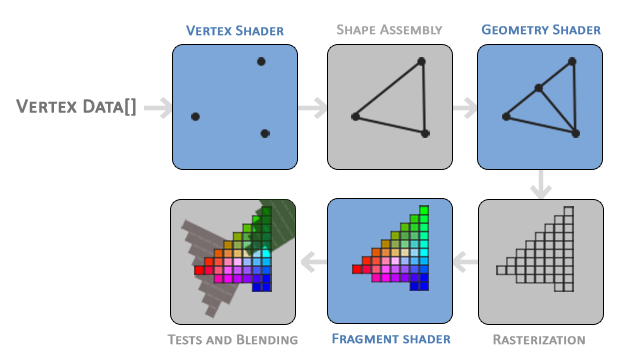
\includegraphics[width=12cm]{pipeline.png}
    }
    \caption{\fontsize{11pt}{1.0cm}\zarbold\textbf{\lr{Graphic pipeline: from learnopengl.com}}}
    \label{fig:my_label}
\end{figure}
\vspace*{0.6cm}

    به طور کلی وظیفه \lr{Vertex Shader} انتقال\footnote{\lr{translate}} یک نقطه از فضای \lr{NDC} به فضای دیگر است، غالبا این فضا\footnote{\lr{3D space}} همان جهان بازی یا برنامه سه بعدی است، برای \lr{Transform} کردن فضای بازی به فضایی دیگر از ماتریس ها استفاده می شود، به طوری که هر فضا دارای یک \lr{Transformation Matrix}  است، برای رسم کردن مثلث ما نیازی به تغییر فضا نداریم و در \lr{NDC} ادامه می دهیم.
    یک \lr{Vertex shader} ساده به صورت زیر است:
    \pagebreak
    \begin{LTR}
    \small
        \begin{lstlisting}[style=C++Style,caption=\lrit{basic vertex shader}]
#version 330 core
layout (location = 0) in vec3 aPos;

void main()
{
    gl_Position = vec4(aPos.x, aPos.y, aPos.z, 1.0);
}
        \end{lstlisting}
    \end{LTR}
    \normalsize
    \vspace*{0.3cm}

    کد بالا ساده ترین مدل برای استفاده از \lr{vertex shader} است، این کد به زبان \lr{GLSL}\footnote{\lr{OpenGL Shading Language}} نوشته شده است، در خط اول نوع ویژگی ها را که پیش تر توضیح داده بودیم
    را مشخص کرده ایم، خط 2 یک متغیر از نوع \lr{vec3} به اسم \lr{aPos} تعریف کرده ایم، با استفاده از \lrit{layout (location = 0)} در این خط مشخص کرده ایم که این متغیر در حافظه\footnote{\lr{memory}} در چه موقعیتی قرار میگیرد، این ویژگی هنگامی که بخواهیم مقادیر دیگری به جز مختصات نقطه، در یک آرایه ذخیره کنیم و به کارت گرافیک دهیم کارایی دارد.
    در نهایت متغیر \lr{(gl\_Position)} که نشان دهنده مکان نقطه در حال پردازش است را به وسیله مقادیری که از کد  \lr{C} خواندیم، مقدار چهارم را برابر 1 قرار می دهیم، مقدار چهارم در این فضا کاربردی ندارد اما در فضای سه بعدی و در \lr{perspective view} به کار ما می آید.\par
    مرحله بعد ساختن یک \lr{Fragment shader} است، وظیفه این بخش از \lr{pipeline} انجام محاسبات و تعیین رنگ پیکسل\footnote{\lr{shading}} می باشد، تمامی محاسبات مربوط به نور، سایه، بازتاب و افکت های گرافیکی غالبا در این مرحله انجام می شود، البته این مقادیر در مراحل بعد ممکن است تغییر کنند.
    یک \lr{fragment shader} ساده به صورت زیر است:

    \begin{LTR}
    \small
        \begin{lstlisting}[style=C++Style,caption=\lrit{basic fragment shader}]
#version 330 core
out vec4 FragColor;

void main()
{
    FragColor = vec4(1.0f, 0.5f, 0.2f, 1.0f);
}
        \end{lstlisting}
    \end{LTR}
    \normalsize
    \vspace*{0.3cm}
    کد بالا مقدار خروجی برای رنگ این \lr{fragment} را برابر با مقداری ثابت قرار می دهد، نوع متغیر \lr{FragColor} از نوع \lr{vec4} تعریف شده و مقادیری که دریافت کرده به ترتیب معنی \lr{red, green, blue, alpha} را می دهند، مقادیر باید بین صفر و یک باشند.\par
    حالا هر کدام از کد های بالارا \lr{compile} می کنیم و سپس به برنامه اصلی که روی \lr{Gpu} قرار می گیرد متصل می کنیم، این برنامه را \lr{shader program} می نامیم، قطعه کد پایین مراحل \lr{compile} و \lr{link} کردن \lr{shader program} را نشان می دهد.

    \begin{LTR}
    \small
        \begin{lstlisting}[style=C++Style,caption=\lrit{compile and link shaders to shader program}]
// hold Vertex shader ID
unsigned int vertexShader;
// create a shader of vertex type
vertexShader = glCreateShader(GL_VERTEX_SHADER);
// upload source code
glShaderSource(vertexShader, 1, &vertexShaderSource, NULL);
// compile vertex shader source
glCompileShader(vertexShader);
// -------------------------------------------------
// hold Fragment shader ID
unsigned int fragmentShader;
//create a shader of frament type
fragmentShader = glCreateShader(GL_FRAGMENT_SHADER);
// upload source
glShaderSource(fragmentShader, 1, &fragmentShaderSource, NULL);
// compile fragment shader source
glCompileShader(fragmentShader);
// -------------------------------------------------
// hold shader program ID
unsigned int shaderProgram;
// create a shader program
shaderProgram = glCreateProgram();
// attach vertex shader to program
glAttachShader(shaderProgram, vertexShader);
// attach fragment shader to program
glAttachShader(shaderProgram, fragmentShader);
glLinkProgram(shaderProgram); // link the program
        \end{lstlisting}
    \end{LTR}
    \normalsize
    \vspace*{0.3cm}

    حالا می توانیم از این \lr{shader program} برای تصویر کردن داده ها استفاده کنیم، در بخش بعد داده ها را بر روی \lr{Gpu} بارگزاری می کنیم.

\newpage
\subsection{\lr{Upload Data to GPU}}
\noindent
\normalsize
    برای استفاده از مشخصات نقاطی که تعریف کردیم باید آن هارا روی \lr{memory} کارت گرافیک آپلود کنیم، انتقال اطلاعات بین \lr{cpu} و \lr{gpu} نسبتا کند است، پس سعی می کنیم اطلاعات هر چه بیشتری را در یک عملیات منتقل کنیم، برای مدیریت حافظه بر روی کارت گرافیک از \lr{vbo}\footnote{\lr{vertex buffer object}} استفاده می کنیم، این بافر\footnote{\lr{Buffer}} ها قابلیت نگهداری تعداد زیادی از داده ها را دارند، برای ساختن یک \lr{buffer} در \lr{opengl} و نگهداری مشخصه بافر ایجاد شده به صورت زیر عمل می کنیم:

    \begin{LTR}
    \small
        \begin{lstlisting}[style=C++Style,caption=\lrit{creating a buffer object}]
unsigned int VBO;
glGenBuffers(1, &VBO);
        \end{lstlisting}
    \end{LTR}
    \normalsize
    \vspace*{0.3cm}

    برای استفاده کردن از این بافر و ارسال اطلاعات باید آن را \lr{bind} کنیم:
    \begin{LTR}
    \small
        \begin{lstlisting}[style=C++Style,caption=\lrit{binding to target gl\_array\_buffer}]
glBindBuffer(GL_ARRAY_BUFFER, VBO);
        \end{lstlisting}
    \end{LTR}
    \normalsize
    \vspace*{0.3cm}

    حالا که بافر \lr{bind} شده است، می توانیم داده هایی که در آرایه \lr{vertices} تعریف کردیم را به \lr{gpu memory} منتقل کنیم:
        \begin{LTR}
    \small
        \begin{lstlisting}[style=C++Style,caption=\lrit{uploading data for static draw}]
glBufferData(GL_ARRAY_BUFFER,
             sizeof(vertices),
             vertices,
             GL_STATIC_DRAW);
        \end{lstlisting}
    \end{LTR}
    \normalsize
    \vspace*{0.3cm}

    اکنون داده های ما بر روی \lr{gpu} قرار گرفته اند، آخرین آرگومانی که به تابع بالا دادیم به این معنی است که این داده ها مستعد تغییر نیستند، یعنی نوشتن بر روی آن ها زیاد صورت نمی گیرد اما باید برای خوانده شدن به سرعت در دسترس باشند زیرا به مراتب خوانده می شوند، این به کارت گرافیک کمک می کند تا داده هارا در جایی از حافظه قرار دهد تا این ویژگی ها را داشته باشد.

    داده هایی که بر روی کارت گرافیک دادیم قرار داده ایم خام هستند، باید برای \lr{vertex shader} مشخص کنیم که به چه صورت باید داده هارا تفسیر کند، برای استفاده از \lr{attribute} ها در \lr{vertex shader} باید نوع تفسیر داده هارا نیز به صورت دستی مشخص کنیم، به اینکار \lr{Linking Vertex Attribute} می گویند.

    \vspace*{0.6cm}
\begin{figure}[ht]
    \centering
    \href{https://learnopengl.com}{
        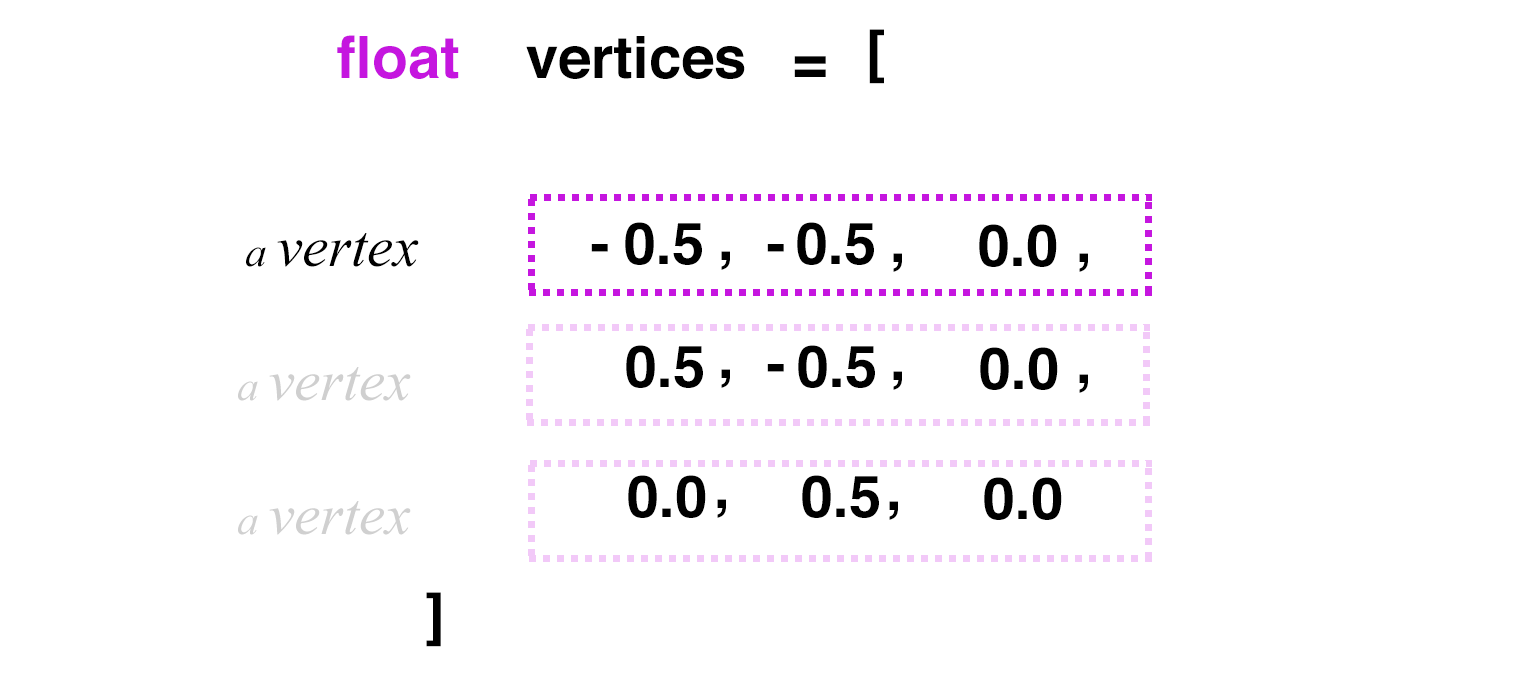
\includegraphics[width=12cm]{images/shm-linking-vertex-attribute.png}
    }
    \caption{\fontsize{11pt}{1.0cm}\zarbold\textbf{\lr{vertex attribute linking}}}
    \label{fig:my_label}
\end{figure}
\vspace*{0.6cm}

    برای انجام اینکار باید مقدار چند ویژگی را بدانیم:
\begin{persian}
    \begin{enumerate}
      \item اولین آرگومان برابر با مقداری است که برای متغیر \lr{aPos} در \lr{vertex shader} به وسیله \lr{layout (location = 0)} مشخص کردیم که در این مورد برابر با صفر است.
      \item آرگومان دوم مشخص کننده تعداد متغیر های است که باید به عنوان یک \lr{vertex} شناسایی شوند، این مقدار برای مثال ما برابر 3 است.
      \item این آرگومان مشخص کننده نوع داده هایی است که بارگزاری شده اند، در این مورد \lr{float} است.
      \item مشخص می کند که داده ها نیاز به نرمال سازی\footnote{\lr{normalize}} دارند یا خیر.
      \item این مقدار مشخص می کند چند بایت داده باید برای این \lr{vertex} خوانده شود، به این مقدار \lr{stride} می گویند.
      \item مقدار آخر در مثال ما کاربرد ندارد، در مثال های بعدی می بینیم که مقادیر مربوط به رنگ و دیگر ویژگی های یک نقطه را در به صورت پیوسته در آرایه \lr{vertices} اضافه می کنیم، آنگاه باید از \lr{offset} برای مشخص کردن هر کدام از این ویژگی ها استفاده کنیم.
    \end{enumerate}
\end{persian}

    شکل 1.3 متناسب با توضیحات ساخته شده.

    \begin{LTR}
    \small
        \begin{lstlisting}[style=C++Style,caption=\lrit{link vertex attribute to vertex data}]
glVertexAttribPointer(
    0, // layout (location = 0)
    3, // 3 value for this vertex exists
    GL_FLOAT, // type of each value in vertex
    GL_FALSE, // no need to normalize data
    3 * sizeof(float), // 3 (size of) float in each vertex
    (void*)0  //no offset
    );

glEnableVertexAttribArray(0);
        \end{lstlisting}
    \end{LTR}
    \normalsize
    \vspace*{0.3cm}

    در پروژه های بزرگ تر انجام دادن این عملیات برای تک تک اشیاء موجود در صحنه \footnote{\lr{3D Scene}}بیهوده و زمان گیر است، برای همین از یکی دیگر از انواع بافر ها به اسم \lr{VAO}\footnote{\lr{vertex array object}} استفاده می کنیم، این بافر تمامی مراحل قبل و فعال سازی \lr{vertex attribute} ها را ذخیره می کند و دفعات بعد دیگر نیازی به انجام تمامی این مراحل نیست و ما فقط باید \lr{VAO} را \lr{bind} کنیم:

    \begin{LTR}
    \small
        \begin{lstlisting}[style=C++Style,caption=\lrit{link vertex attribute to vertex data}]
unsigned int VAO;
glGenVertexArrays(1, &VAO);
// 2. copy our vertices array in a buffer for OpenGL to use
glBindBuffer(GL_ARRAY_BUFFER, VBO);
glBufferData(GL_ARRAY_BUFFER, sizeof(vertices), vertices, GL_STATIC_DRAW);
// 3. then set our vertex attributes pointers
glVertexAttribPointer(0, 3, GL_FLOAT, GL_FALSE, 3 * sizeof(float), (void*)0);
glEnableVertexAttribArray(0);

        \end{lstlisting}
    \end{LTR}
    \normalsize
    \vspace*{0.3cm}


    حالا می توانیم با استفاده \lr{shader program} و \lr{vao} مثلث را بر روی صفحه\footnote{\lr{Display device}} رسم کنیم، این کار را در بخش بعدی انجام می دهیم.

\newpage
\subsection{\lr{Render Loop}}
\noindent
\normalsize
    در بخش های قبل داده هارا بر روی کارت گرافیک قرار دادیم و \lr{shader} هارا کامپایل و لینک کردیم، حالا برای رسم کردن مثلث نیاز به کدهای زیر داریم:

    \begin{LTR}
    \small
        \begin{lstlisting}[style=C++Style,caption=\lrit{link vertex attribute to vertex data}]
glUseProgram(shaderProgram); // bind the shader program
glBindVertexArray(VAO);
glDrawArrays(GL_TRIANGLES, 0, 3);
        \end{lstlisting}
    \end{LTR}
    \normalsize
    \vspace*{0.3cm}

    ابتدا \lr{shader program} را فعال می کنیم، سپس \lr{VAO} که ساختیم را \lr{bind} می کنیم، حالا تمامی داده ها و تفسیر ها آماده هستند، برای رسم از تابع خط آخر می خواهیم که با داده ها تشکیل مثلث بدهد، ابتدای و انتهای بایت هایی که باید از \lr{vertex array} بخواند را مشخص می کنیم، پس از کامپایل کردن و اجرای برنامه با شکل زیر رو به رو می شویم.

\vspace*{0.3cm}
\begin{figure}[ht]
    \centering
    \href{https://learnopengl.com}{
        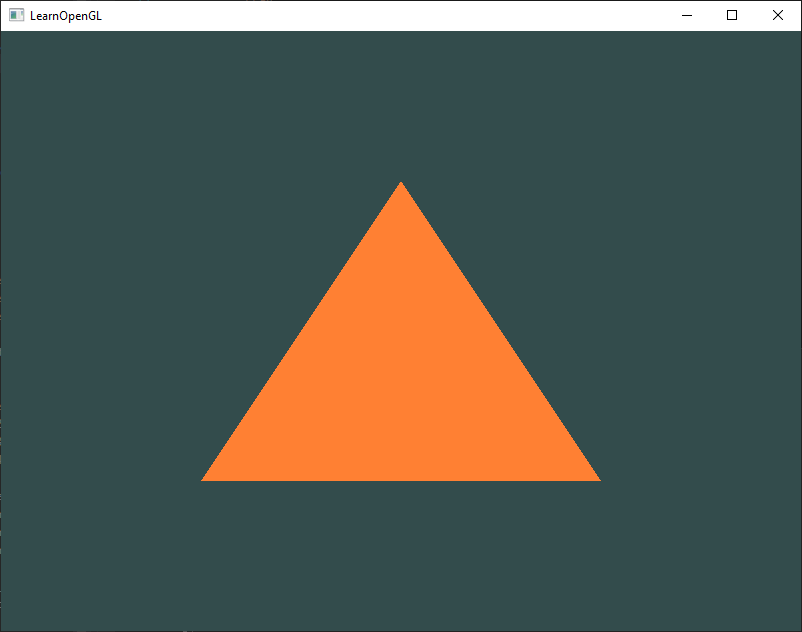
\includegraphics[width=10cm]{images/hellotriangle.png}
    }
    \caption{\fontsize{11pt}{1.0cm}\zarbold\textbf{\lr{hello triangle}}}
    \label{fig:my_label}
\end{figure}
\vspace*{0.3cm}

\newpage
    برای اینکه بتوانیم دیگر ویژگی های مدل هارا به کارت گرافیک ارسال کنیم و از آن ها استفاده کنیم می توانیم از چند \lr{attribute} یا از نوعی از متغیر ها به اسم \lr{uniform} استفاده کنیم، در ابتدا برای افزودن رنگ به هر کدام از \lr{vertex} ها از \lr{attribute} های \lr{vertex shader} استفاده می کنیم، برای این کار کد \lr{vertex shader}  را به شکل زیر تغییر می دهیم:

    \begin{LTR}
    \small
        \begin{lstlisting}[style=C++Style,caption=\lrit{declare and use aColor}]
#version 330 core
layout (location = 0) in vec3 aPos;
layout (location = 1) in vec3 aColor

out vec3 ourColor;

void main()
{
    gl_Position = vec4(aPos, 1.0);
    ourColor = aColor
}
        \end{lstlisting}
    \end{LTR}
    \normalsize
    \vspace*{0.3cm}

    و کد \lr{fragment shader} را به شکل زیر می نویسیم تا بتوانیم از مقادیر رنگ استفاده کنیم:
    \begin{LTR}
    \small
        \begin{lstlisting}[style=C++Style,caption=\lrit{render fragment with color from vertex shader}]
#version 330 core
out vec4 FragColor;
in vec3 ourColor;

void main()
{
    FragColor = vec4(ourColor, 1.0);
}
        \end{lstlisting}
    \end{LTR}
    \normalsize
    \vspace*{0.3cm}

    حالا داده های مربوط به رنگ هر \lr{vertex} را در انتهای داده های مربوط به همان \lr{vertex} اضافه می کنیم، کد به شکل زیر تغییر می کند:
    \begin{LTR}
    \small
        \begin{lstlisting}[style=C++Style,caption=\lrit{position and color data in one array}]
float vertices[] = {
    // positions         // colors
     0.5f, -0.5f, 0.0f,  1.0f, 0.0f, 0.0f,   // bottom right
    -0.5f, -0.5f, 0.0f,  0.0f, 1.0f, 0.0f,   // bottom left
     0.0f,  0.5f, 0.0f,  0.0f, 0.0f, 1.0f    // top
};
        \end{lstlisting}
    \end{LTR}
    \normalsize
    \vspace*{0.3cm}

    داده هارا به شکل قبل به \lr{VBO} اضافه می کنیم، سپس \lr{VAO} را \lr{bind} می کنیم، یک مرحله جدید در \lr{link vertex attribute} برای رنگ ها اضافه شده است، این مرحله به شکل زیر است:
       \begin{LTR}
    \small
        \begin{lstlisting}[style=C++Style,caption=\lrit{position and color data in one array}]
// position attribute
glVertexAttribPointer(0, 3, GL_FLOAT, GL_FALSE, 6 * sizeof(float), (void*)0);
glEnableVertexAttribArray(0);
// color attribute
glVertexAttribPointer(1, 3, GL_FLOAT, GL_FALSE, 6 * sizeof(float), (void*)(3* sizeof(float)));
glEnableVertexAttribArray(1);
        \end{lstlisting}
    \end{LTR}
    \normalsize
    \vspace*{0.3cm}

    همانطور که می بینیم در این مرحله متغیر های مربوط \lr{stride} و \lr{offset} به شکل جدید برای استفاده از و تفسیر تمام داده برای \lr{gpu} تغییر کرده اند، در خط 5 کد بالا متغیر \lr{offset} نشان دهنده این است که برای خواندن سه مقدار برای رنگ، باید \lr{offset} را برابر 3 قرار دهیم تا سه مقدار اول که برای داده های مکان نقطه تعریف کرده ایم در نظر نگیرد، همچنین متغیر \lr{stride} را برابر با شش قرار دادیم، این به معنی این است که هر 6 مقدار در آرایه بیانگر ویژگی ها برای یک نقطه متفاوت است.\par
    رنگ مثلث به صورت زیر تغییر می کند:
\newpage
\vspace*{0.3cm}
\begin{figure}[ht]
    \centering
    \href{https://github.com/devprofile98/shm}{
        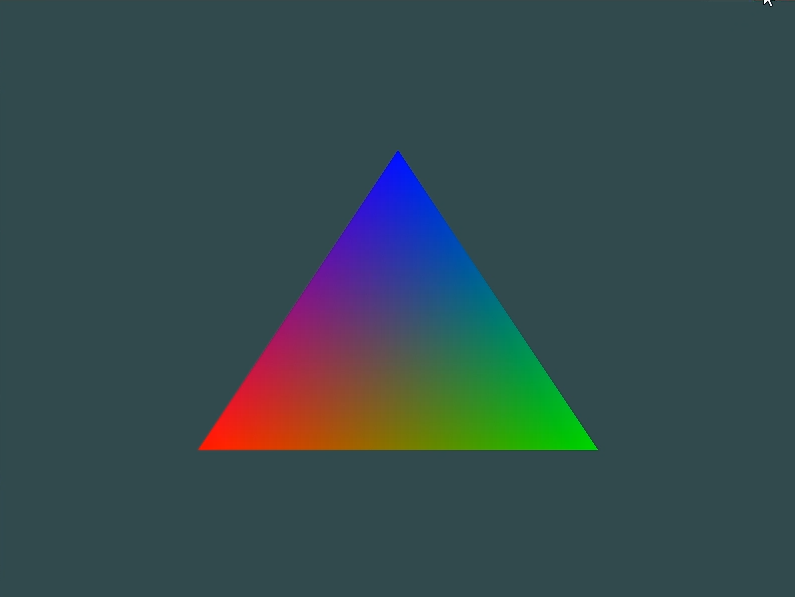
\includegraphics[width=10cm]{images/colorfultriangle.png}
    }
    \caption{\fontsize{11pt}{1.0cm}\zarbold\textbf{\lr{colorful triangle}}}
    \label{fig:my_label}
\end{figure}
\vspace*{0.3cm}
    در مثال بالا \lr{opengl} مقدار رنگ سه نقطه را از ما دریافت کرد و به صورت خودکار مقدار رنگ بین این نقاط را به صورت یک درون یابی خطی\footnote{\lr{Linear Interpolation}} مشخص کرد.\par
    این روش برای مدل\footnote{\lr{3D Models}} ها و اشیاء سه بعدی نه تنها کاربردی نیست بلکه هزینه زیادی دارد، روش بهتر برای مقدار دهی به رنگ و ایجاد جزئیات برای اشیاء استفاده از تکسچر\footnote{\lr{texture}} ها است، در بخش بعد درباره تکسچرها توضیح می دهم.

\newpage
\subsection{\lr{Textures}}
\noindent
\normalsize
    تصور کنید می خواهیم یک دیوار را شبیه سازی کنیم، دیوار را می توانیم با چهار نقطه با استفاده از \lr{EBO}\footnote{\lr{element buffer object}} بسازیم، این چهار نقطه با توجه به مقدار نقاط تشکیل یک چهارضلعی می دهند. مرحله بعد اضافه کردن جزئیات رنگ، یعنی تصویر آجر ها بر روی دیوار است، این کار به سادگی امکان پذیر نیست، زیرا ما فقط قابلیت تعیین چهار رنگ برای چهار نقطه را داریم، پس نمی توانیم با چهار رنگ و \lr{linear interpolation} که \lr{opengl} بین این رنگ ها انجام می دهد یک دیوار آجری رندر کنیم، راه حل این مشکل استفاده از یک \lr{texture} است، به صورت ساده می توانیم عکس یک دیوار آجری را به \lr{opengl} بدهیم و بخواهیم که به ازای هر \lr{fragment} از یکی از \lr{pixel} های عکسی که ما به عنوان \lr{texture} آپلود کرده ایم استفاده کند. برای استفاده از یک \lr{texture} ما باید مراحل زیر را انجام دهیم.

\begin{persian}
    \begin{enumerate}
      \item اضافه کردن \lr{texture coordinates} به آرایه داده ها و آپلود داده ها بر روی \lr{vertex attribute}.
      \item خواندن عکس از حافظه و آپلود کردن آن بر روی \lr{Gpu}.
      \item تنظیم کردن حداقل برخی از ویژگی های تکسچر که به صورت پیشفرض مقداری ندارند.
      \item استفاده از توابع \lr{GLSL} برای نگاشت\footnote{\lr{sample}} کردن \lr{texture}
    \end{enumerate}
\end{persian}

    در مرحله اول مقادیر \lr{texture coordinate} را به آرایه داده ها اضافه می کنیم:
    \begin{LTR}
    \small
        \begin{lstlisting}[style=C++Style,caption=\lrit{position and color data in one array}]
float vertices[] = {
    // positions          // colors           // texture coords
     0.5f,  0.5f, 0.0f,   1.0f, 0.0f, 0.0f,   1.0f, 1.0f,
     0.5f, -0.5f, 0.0f,   0.0f, 1.0f, 0.0f,   1.0f, 0.0f,
    -0.5f, -0.5f, 0.0f,   0.0f, 0.0f, 1.0f,   0.0f, 0.0f,
    -0.5f,  0.5f, 0.0f,   1.0f, 1.0f, 0.0f,   0.0f, 1.0f
};
        \end{lstlisting}
    \end{LTR}
    \normalsize
    \vspace*{0.3cm}

    دقت کنید که باید مراحل \lr{linking vertex attribute} را برای مقادیر جدید انجام دهیم.

    حالا عکس را از دیسک می خوانیم، برای این کار از \href{https://github.com/nothings/stb}{\lrbold{stbi\_image}} استفاده می کنیم، این کتابخانه به صورت \lr{single header library} در دسترس است، این گونه کتابخانه در یک فایل نوشته شده اند و استفاده درست از آن ها با استفاده از ماکرو\footnote{\lr{macro}} هاست.

    پس از بازکردن عکس در کد باید یک \lr{texture} بسازیم، ابتدا یک شئ\lr{texture} می سازیم و سپس می توانیم داده هایی را که از عکس  خواندیم را بر روی آن \lr{upload} کنیم، اینکار به شیوه زیر انجام می گیرد:

    \begin{LTR}
    \small
        \begin{lstlisting}[style=C++Style,caption=\lrit{load and upload data to gpu}]
unsigned int texture; // hold texture ID
glGenTextures(1, &texture); // create texture object on gpu
// bind texture to 2d_texture target
glBindTexture(GL_TEXTURE_2D, texture);
// upload image data to texture that is bound i.e texture variable
glTexImage2D(GL_TEXTURE_2D, 0, GL_RGB, width, height,
    0, GL_RGB, GL_UNSIGNED_BYTE, data); // data is the Image
// generating mip maps for this texture
glGenerateMipmap(GL_TEXTURE_2D);
        \end{lstlisting}
    \end{LTR}
    \normalsize
    \vspace*{0.3cm}


    نیاز داریم که برخی مقادیر را برای \lr{texture} تنظیم کنیم در غیر اینصورت با یک تکسچر سیاه رو به رو می شویم، مقادیر زیر برای تنظیم تکرار شدن تصویر\footnote{\lr{repeat}} در جهات مختلف و مشخص کردن الگوریتم مناسب برای زمان کوچک نمایی\footnote{\lr{Minifying}} یا بزرگ نمایی\footnote{\lr{Magnifying }} تصویر است، به صورت زیر این مقادیر را تنظیم می کنیم:

    \begin{LTR}
    \small
        \begin{lstlisting}[style=C++Style,caption=\lrit{set minimum setting for a texture}]
glTexParameteri(GL_TEXTURE_2D, GL_TEXTURE_WRAP_S, GL_REPEAT);	
glTexParameteri(GL_TEXTURE_2D, GL_TEXTURE_WRAP_T, GL_REPEAT);
glTexParameteri(GL_TEXTURE_2D, GL_TEXTURE_MIN_FILTER, GL_LINEAR_MIPMAP_LINEAR);
glTexParameteri(GL_TEXTURE_2D, GL_TEXTURE_MAG_FILTER, GL_LINEAR);
        \end{lstlisting}
    \end{LTR}
    \normalsize
    \vspace*{0.3cm}

    مختصات تکسچر را در \lr{vertex shader} به صورت یک \lr{vertex attribute} جدید تعریف می کنیم و به مرحله \lr{fragment shader} می فرستیم، ارسال این داده ها بین مراحل مختلف \lr{pipeline} را با استفاده از متغیر هایی که با \lr{in} یا\lr{out} تعریف می شوند انجام می دهیم، به این صورت که متغیر را در مرحله ای که زودتر انجام می شود(در این مورد \lr{vertex shader}) به صورت \lr{out} تعریف می کنیم و در مرحله بعد آن را با \lr{in} تعریف می کنیم، دقت کنید باید نام متغیر دقیقا برابر باشد، کد زیر به \lr{vertex shader} اضافه می کنیم:

       \begin{LTR}
    \small
        \begin{lstlisting}[style=C++Style,caption=\lrit{vertex shader to use texture}]
layout (location = 2) in vec2 aTexCoord;
out vec2 TexCoord; // vec2 because of 2d image
...
void main()
{
    ....
    TexCoord = aTexCoord;
}
        \end{lstlisting}
    \end{LTR}
    \normalsize
    \vspace*{0.3cm}

    در قمست \lr{fragment shader} نیز کد به شکل زیر تغییر می کند:

    \begin{LTR}
    \small
        \begin{lstlisting}[style=C++Style,caption=\lrit{fragment shader to use texture}]
#version 330 core
out vec4 FragColor;
...
in vec2 TexCoord;

uniform sampler2D ourTexture;

void main()
{
    //built in texture function for sampling texture to fragment
    FragColor = texture(ourTexture, TexCoord);
}
        \end{lstlisting}
    \end{LTR}
    \normalsize
    \vspace*{0.3cm}

    نتیجه به شکل زیر در می آید:

\vspace*{0.3cm}
\begin{figure}[ht]
    \centering
    \href{https://github.com/devprofile98/shm}{
        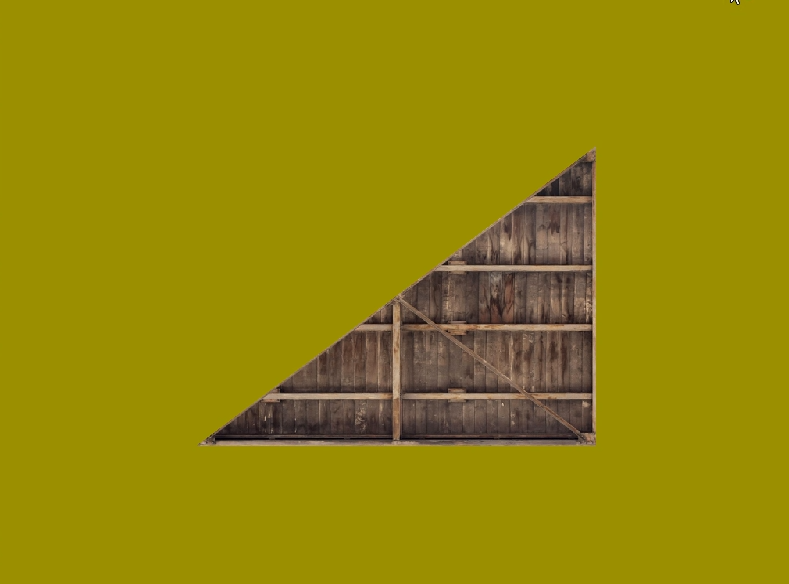
\includegraphics[width=13cm]{images/texturedtriangle.png}
    }
    \caption{\fontsize{11pt}{1.0cm}\zarbold\textbf{\lr{textured triangle}}}
    \label{fig:my_label}
\end{figure}
\newpage


% end of section -------------------

% section start --------------------
% \vspace*{6.0cm}
%\addcontentsline{toc}{section}{دوربین و حرکت در جهان}
\section{\fontsize{15pt}{1.0cm}\zarbold\textbf{دوربین و حرکت در جهان}}
\vspace*{0.6cm}
\subsection{\lr{Transformations}}
\noindent
\normalsize

    می توانیم با دو مثلث یک مربع درست کنیم، و با شش مربع یک مکعب تشکیل دهیم، و با استفاده از یک حلقه و چند \lr{draw call} چند مکعب بسازیم، اما در حال حاظر این کار بی فایده است زیرا تمامی مکعب ها بر روی یکدیگر قرار می گیرند و ما تنها یک مکعب را به صورت دو بعدی می بینیم، برای دیدن یک مکعب به یک محیط که شبیه ساز سه بعد باشد نیاز داریم، می توانیم مکان\footnote{\lr{position}} مکعب هارا در حلقه تغییر دهیم و در قسمت های مختلف صفحه رندر کنیم، به این کار \lr{translate} کردن می گوییم، این عمل را با استفاده از یک ماتریس
    $4x4$
    انجام می دهیم، یک \lr{translation matrix} به شکل زیر است:\par
\begin{center}
\setlength\arraycolsep{5pt}
\renewcommand{\arraystretch}{0.75}
	$$
	\begin{bmatrix}
	1 & 0 & 0 & x \\
	0 & 1 & 0 & y \\
	0 & 0 & 1 & z \\
    0 & 0 & 0 & 1
	\end{bmatrix}
	\quad
	$$
\end{center}

    مقادیر $(x, y, z)$ به ترتیب نشان دهنده تغییرات در راستای بردار متناسب با خود هستند، می توانیم هر کدام از نقاط مدل خود را توسط ماتریس بالا به نقطه جدید خود منتقل کنیم، ماتریس های \lr{rotation} و \lr{scale} نیز به ترتیب برای چرخش حول محور های مشخص و تغییر مقیاس استفاده می شوند، به حاصل ضرب این سه جزء یک \lr{model matrix} می گویند.\par
    پس از ضرب کردن \lr{model matrix} در مختصات هر نقطه از شئ سه بعدی، اصطلاحا مختصات نقاط را در \lr{local space} به \lr{world space} برده ایم.\par
    برای انجام عملیات ریاضی مربوط به \lr{opengl} بر روی \lr{cpu} از کتابخانه \lrbold{GLM} استفاده می کنیم، این کتابخانه دارای کلاس ها و توابعی است که نمایانگر ساختار های ریاضیاتی مانند \lr{vector} ها و \lr{matrix} ها است، همچنین تعداد دیگری از توابع را داراست که برای ساده سازی کار ما فراهم شده اند، یکی از این توابع \lr{glm::LookAt} است، می  توانیم از این کلاس برای تشکیل یک \lr{view matrix} استفاده کنیم که نشانگر \lrbold{Camera}  است.\par
    \vspace*{0.6cm}
    \subsubsection{\lr{Camera}}
    \vspace*{0.3cm}

    در جهان واقعی اگر جسمی به نسبت دیگر اجسام از ما فاصله بیشتری داشته باشد کوچکتر دیده می شود، این تعریف بسیار ساده و مختصری از \lr{perspective view} است، نور بازتاب شده از اجسام به مرکز چشم ما برمیگردد و اجسامی که نزدیک تر هستند بزرگتر دیده می شوند، در مقابل این مدل \lr{orthographic views } قرار دارند، این مدل در طراحی های صنعتی بیشتر کاربر دارد و در جهان ما وجود ندارد، هر کدام از \lr{pixel} های صفحه پرتویی\footnote{\lr{Ray}} به صورت جداگانه از خود ساطع می کنند و در نتیجه باعث از بین رفتن تصویر روزمره ما می شوند، همه این پرتوها موازی هستند و در نتیجه فاصله جسم از بیننده در نحوه دیدن شکل تاثیری ایجاد نمی کند، ما برای داشتن یک فضای سه بعدی واقع گرایانه از \lr{perspective projection} استفاده می کنیم، برای ساختن این ماتریس از \lr{GLM} به شکل زیر استفاده می کنیم:

    \begin{LTR}
    \small
        \begin{lstlisting}[style=C++Style,caption=\lrit{fragment shader to use texture}]
glm::mat4 proj = glm::perspective(
    glm::radians(45.0f),
    (float)width/(float)height,
    0.1f, 100.0f);
        \end{lstlisting}
    \end{LTR}
    \normalsize
    \vspace*{0.3cm}

    آرگومان اول مقدار \lr{FOV}\footnote{\lr{field of view}} است، این مقدار به نحوی مقدار بزرگنمایی تصویر ما را مشخص می کند، آرگومان دوم نسبت ابعاد صفحه\footnote{\lr{aspect ratio}} است، مقادیر سوم و چهارم به ترتیب فاصله صفحه نزدیک و دور\footnote{\lr{Far/Near Plane}} را مشخص می کنند، این مشخصات تشکیل یه فضای سه بعدی برش داده شده\footnote{\lr{Clip Space}} را می دهند که هر چه خارج از آن باشد قابل مشاهده نیست، همچنین دید \lr{perspective} را به ما ارائه می کنند.
    شکل زیر بیانگر این موضوع است.

\begin{figure}[ht]
    \centering
    \href{https://learnopengl.com}{
        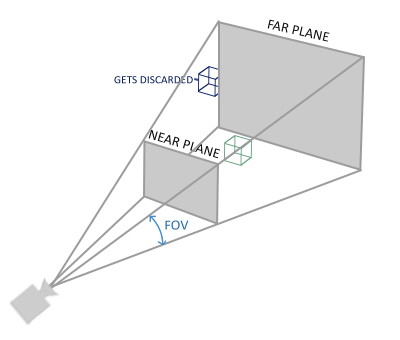
\includegraphics[width=10cm]{images/perspective_frustum.png}
    }
    \caption{\fontsize{11pt}{1.0cm}\zarbold\textbf{\lr{perspective frustum}}}
    \label{fig:perspectiveview}
\end{figure}

    حالا که سه ماتریس \lr{model}, \lr{view} و \lr{projection} را در اختیار داریم می توانیم با ضرب کردن مقدار \lr{(x, y, z, 1)} به ازای هر نقطه، آن را به \lr{clip space} ببریم، به ترتیب با ضرب کردن هر یک از ماتریس هایی که پیش تر گفت شد به \lr{world space} سپس \lr{view space} و در آخر به \lr{clip space} می رویم، همچنین \lr{projection matrix} در نهایت تمامی مقادیر را به \lr{NDC} نیز منتقل می کند.\par
    مقدار تمامی ماتریس های بالا را با استفاده از متغیر های \lr{uniform} به \lr{vertex shader} انتفال می دهیم، مقادیری از این سه ماتریس را که نیاز به تغییر داشته باشند در هر مرتبه اجرای \lr{render loop} دوباره بارگزاری می کنیم.\par
    \lr{vertex shader} به شکل زیر در می آید:
    \begin{LTR}
    \small
        \begin{lstlisting}[style=C++Style,caption=\lrit{going 3D}]
#version 330 core
layout (location = 0) in vec3 aPos;
...
uniform mat4 model;
uniform mat4 view;
uniform mat4 projection;

void main()
{
    // note that we read the multiplication from right to left
    gl_Position = projection * view * model * vec4(aPos, 1.0);
    ...
}
        \end{lstlisting}
    \end{LTR}
    \normalsize
    \vspace*{0.3cm}

    به صورت پیش فرض \lr{opengl} نمی تواند مشخص کند که کدام قسمت از مدل هایی که رندر کرده در تصویر نهایی جلوتر یا عقب تر باید باشند، یعنی امکان دارد قسمت پشت مکعب به جای قسمت جلوی آن رندر شود، در واقع هر کدام از \lr{fragment} ها که دیر تر رندر شوند، بر دیگر \lr{fragment} هایی که در آن پیکسل از قبل رندر شده اند پیروز می شوند و نمایش داده می شوند، برای حل این مشکل از \lr{z-buffer} استفاده می کنیم، \lr{GLFW} به صورت پیش فرض این \lr{buffer} را برای ما ساخته، برای فعال سازی آن دستور زیر را پیش از \lr{render loop} قرار می دهیم:

    \begin{LTR}
    \small
        \begin{lstlisting}[style=C++Style,caption=\lrit{enabling depth buffer}]
glEnable(GL_DEPTH_TEST);
        \end{lstlisting}
    \end{LTR}
    \normalsize
    \vspace*{0.3cm}

    و در انتهای \lr{render loop} نیز دستور زیر را قرار می دهیم:

        \begin{LTR}
    \small
        \begin{lstlisting}[style=C++Style,caption=\lrit{clearing depth buffer for next frame}]
glClear(GL_COLOR_BUFFER_BIT | GL_DEPTH_BUFFER_BIT);
        \end{lstlisting}
    \end{LTR}
    \normalsize
    \vspace*{0.3cm}

    خروجی به شکل زیر خواهد بود:
    \begin{figure}[ht]
    \centering
    \href{https://github.com/devprofile98/shm}{
        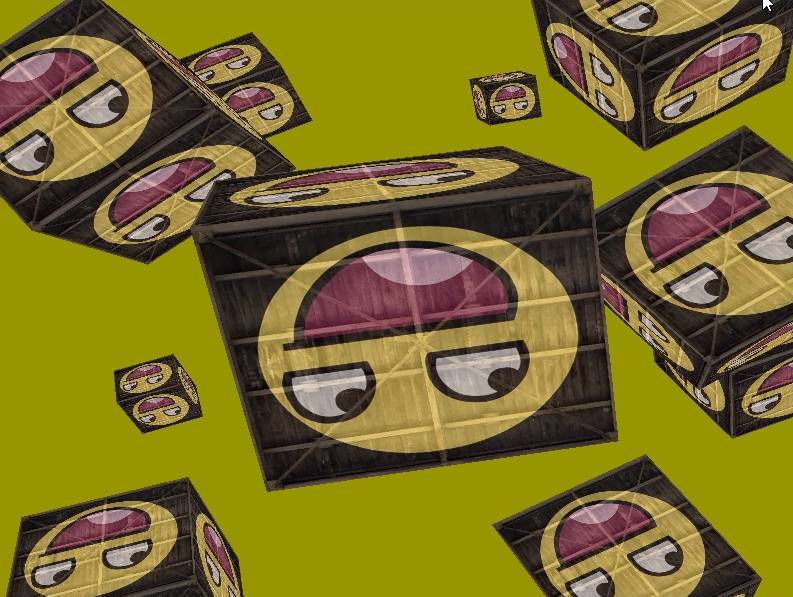
\includegraphics[width=13cm]{images/3d.png}
    }
    \caption{\fontsize{11pt}{1.0cm}\zarbold\textbf{\lr{cubes in 3D}}}
    \label{fig:my_label}
\end{figure}
% end of section ---------------------

% new section ------------------------
\newpage
%\addcontentsline{toc}{section}{نورپردازی و سایه ها}
\section{\fontsize{15pt}{1.0cm}\zarbold\textbf{نورپردازی و سایه ها}}
\vspace*{0.6cm}
\noindent
\normalsize

    به صورت کلی در این پروژه سه مدل منبع نور\footnote{\lr{Light Caster}} پیاده سازی شده است که به ترتیب منابع نور\lr{Directional}, \lr{point} و \lr{spot} می باشند.
\subsection{\lr{Directional Lights}}
    به صورت ساده این گونه از نور را مشابه به نوری در نظر می گیریم که منبع آن در بی نهایت قرار دارد، این فرض باعث می شود که تمامی پرتو های آن تقریبا با هم موازی باشند، خورشید را یک \lr{directional light} در نظر می گیریم. برای بیان کردن این مدل از نور تنها نیاز به سه مولفه
    $(x, y, z)$
    داریم تا بتوانیم یک جهت را در فضای سه بعدی مشخص کنیم که همان جهت پرتو های نور می باشد.\par
    انواع دیگر نور به این شکل ساده نیستند و از ویژگی های دیگری نیز برخوردارند، برای مثال \lr{point light} دارای یک مولفه سه بعدی \lr{position} است، همچنین برای این که میرایی\footnote{\lr{attenuation}} نور را شبیه سازی کنیم از سه مقدار دیگر به عنوان \lr{constant}, \lr{linear} و \lr{quadratic} نیز استفاده می کنیم تا بتوانیم تقریبا میرایی نور به نسبت فاصله از منبع نور را شبیه سازی کنیم. به همین صورت مقادیر دیگری از جمله \lr{direction} را نیز داراست تا به کمک \lr{cut off} بتواند یک نور میرا که در جهت و زاویه خاصی در حال تابیدن است را شبیه سازی کند.

\subsection{\lr{Lighting models}}
    پیاده سازی و شبیه سازی رفتار واقعی نور کاری بسیار پیچیده است که قدرت سخت افزاری و هزینه زیادی را در بردارد، برای همین ما از روش هایی استفاده می کنیم که به صورت تقریبی بتوانند رفتار نور را به صورتی که ما از فیزیک می دانیم شبیه سازی کنند، برای شبیه سازی رفتار نور و برخورد آن با محیط از روش هایی مانند \lr{lambertian} و \lr{blinn-phong} استفاده می شود.

    \subsubsection{\lr{Lambertian}}
        این روش بر اساس زاویه تابش نور با سطح جسم عمل می کند، بدینگونه که اگر سطح عمود به جهت نور باشد تقریبا تمام انرژی نور را دریافت می کند، اگر سطح به صورت موازی با جهت نور قرار داشته باشد مقدار انرژی دریافتی از منبع نور برابر صفر خواهد بود، بقیه حالات قرارگیری این دو نسبت به بسته به
        $\cos \theta$
        مقدار دهی می شود. این روش مستقل از مکان تماشاگر\footnote{\lr{Viewer Eye Dependent}} است، در دنیای واقعی معمولا بسته به \lr{material} استفاده شده در جسم امکان بازتاب و درخشش بیشتر نور از سطح در زاویه های به خصوصی وجود دارد، روش \lr{phong} و بعد تر \lr{blinn} این ویژگی را در خود جای دادند.

    \subsubsection{\lr{Blinn-Phong}}
        این مدل متشکل از سه بخش اصلی است:\par
    \lrbold{ambient}:
    همانطور که در مدل \lr{lambertian} دیدیم، اگر بردار نرمال سطحی عمود بر جهت نور باشد، آن سطح هیچ مقداری از نور را دریافت نمی کند و کاملا تاریک خواهد ماند، این حالت در جهان واقعی نیز در مکان های کاملا بسته اتفاق می افتد و در دیگر حالات مقدار کمی نور از منابع مختلف باعث دیده شدن جسم می شوند، ما در این مدل مقداری از رنگ هر جسم را بدون توجه به زاویه تابش نور به آن جسم می دهیم، این باعث می شود که اجسام کاملا تاریک به وجود نیایند، به این مقدار \lr{ambient color} می گوییم.\par

    \lrbold{diffuse}:
    این مقدار برابر با همان مقداری است که در مدل \lr{lambertian} نیز محاسبه کرده بودیم، بسته به جهت بردار نرمال سطح و جهت نور مقداری انرژی توسط هر سطح جذب می شود و باعث روشن شدن سطح می گردد.\par

    \lrbold{specular}:
    این مقدار باعث به وجود آمدن درخشندگی و بازتاب بیشتر نور نسبت به مکان ناظر می شود، این مقدار مستقل از مکان ناظر نیست، اگر بردار \lr{view direction} در جهت بردار بازتاب نور باشد از حداکثر درخشندگی و \lr{highlight} برخوردار می شود، برای محاسبه کردن جهت بازتاب از تابع \lr{reflect} در \lr{GLSL} استفاده می کنیم، سپس برای محاسبه مقدار بازتاب از ضرب داخلی\footnote{\lr{Dot Product}} بین بردار \lr{view direction} و \lr{reflectDir} استفاده می کنیم، همچنین برای اینکه از منفی شدن مقادیر جلوگیری کنیم از تابع \lr{max} نیز استفاده می کنیم:


    \begin{LTR}
    \small
        \begin{lstlisting}[style=C++Style,caption=\lrit{calculating specular component}]
vec3 viewDir = normalize(viewPos - FragPos);
vec3 reflectDir = reflect(-lightDir, norm);
float spec = pow(max(dot(viewDir, reflectDir), 0.0), 32);
        \end{lstlisting}
    \end{LTR}
    \normalsize
    \vspace*{0.3cm}

    مقدار 32 در کد بالا را مقدار \lr{shininess} می گویند، هر چقدر این مقدار بیشتر باشد درخشش بازتاب در آن نقطه بیشتر می شود.\par
    در نهایت با جمع بستن این سه مقدار می توانیم تقریبی از رفتار نور در دنیای واقعی داشته باشیم، در این پروژه از روش \lr{blinn-phong} استفاده شده.
    نتیجه استفاده از این روش به صورت تصاویر صفحه بعد است.

\begin{figure}[H]
    \centering
    \href{https://github.com/devprofile98/shm}{
        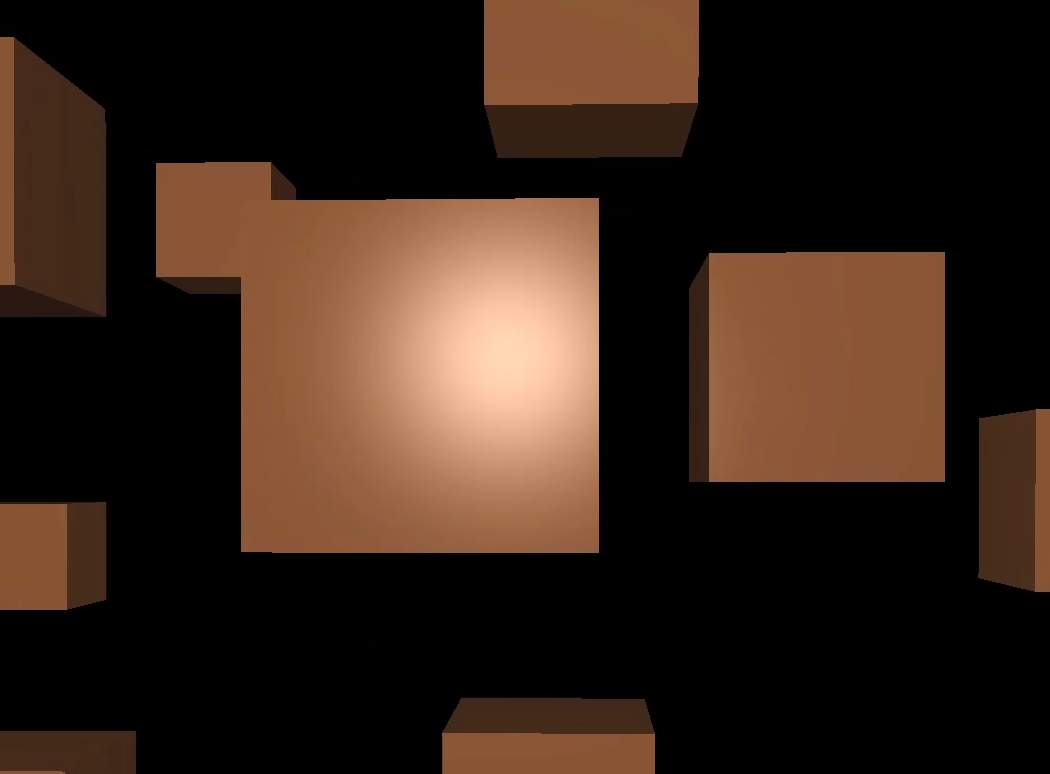
\includegraphics[width=11cm]{images/phong1.png}
    }
    \caption{\fontsize{11pt}{1.0cm}\zarbold\textbf{\lr{blinn-phong shading}}}
    \label{fig:blin}
\end{figure}

\begin{figure}[H]
    \centering
    \href{https://github.com/devprofile98/shm}{
        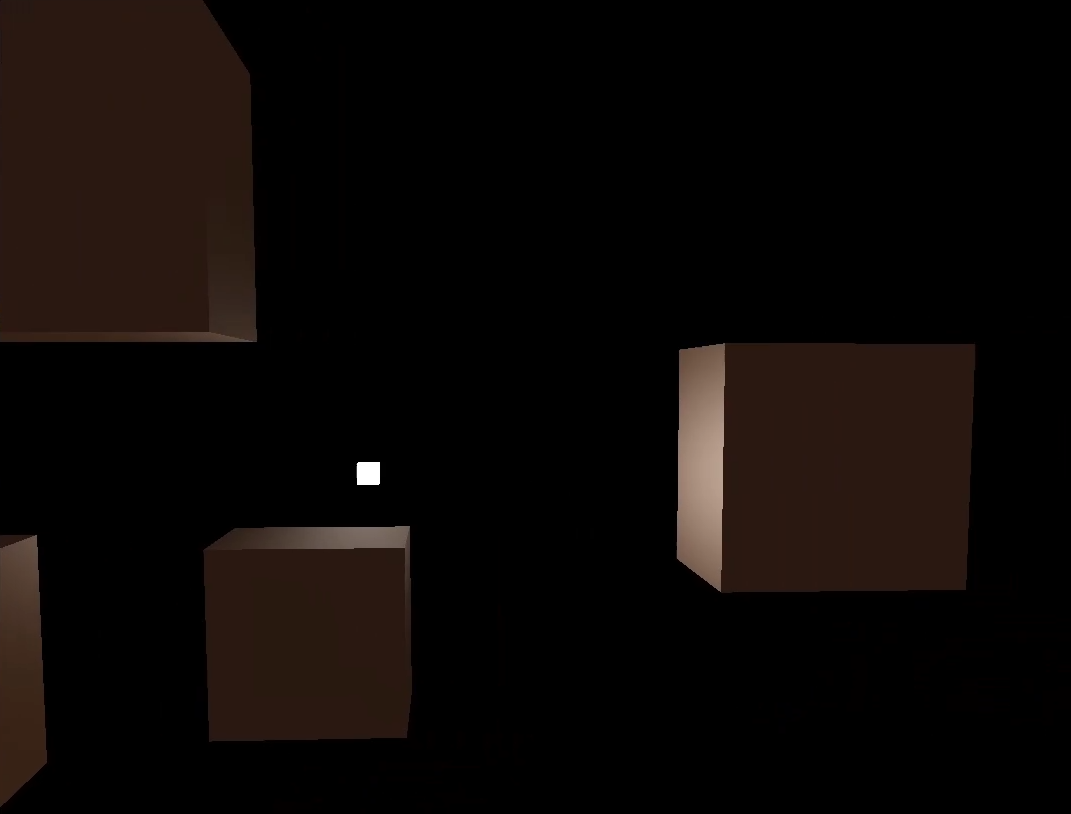
\includegraphics[width=11cm]{images/phong2.png}
    }
    \caption{\fontsize{11pt}{1.0cm}\zarbold\textbf{\lr{blinn-phong shading}}}
    \label{fig:my_label}
\end{figure}

    در حال حاظر تمام سطوح مقداری که بازتاب می کنند تنها به میزان زاویه آن ها با منبع نور بستگی دارد، برای این که بتوانیم این بازتاب را کنترل کنیم و سطوحی با میزان بازتاب متفاوت را تشکیل دهیم، نیاز به جزئیات بیشتری از یک سطح داریم، همانگونه که قبل تر از \lr{texture} ها برای ایجاد جزئیات روی سطوح استفاده کردیم این بار نیز از نوع دیگری از تکسچر ها برای اینکار استفاده می کنیم، به این تکسچر ها \lr{specular map} می گوییم، برای گرفتن مقادیر برای هر پیکسل دقیقا مانند \lr{texture} ها کار می کنیم، یک نمونه از \lr{specular map} به شکل زیر است:\par
\begin{figure}[H]
    \centering
    \href{https://github.com/devprofile98/shm}{
        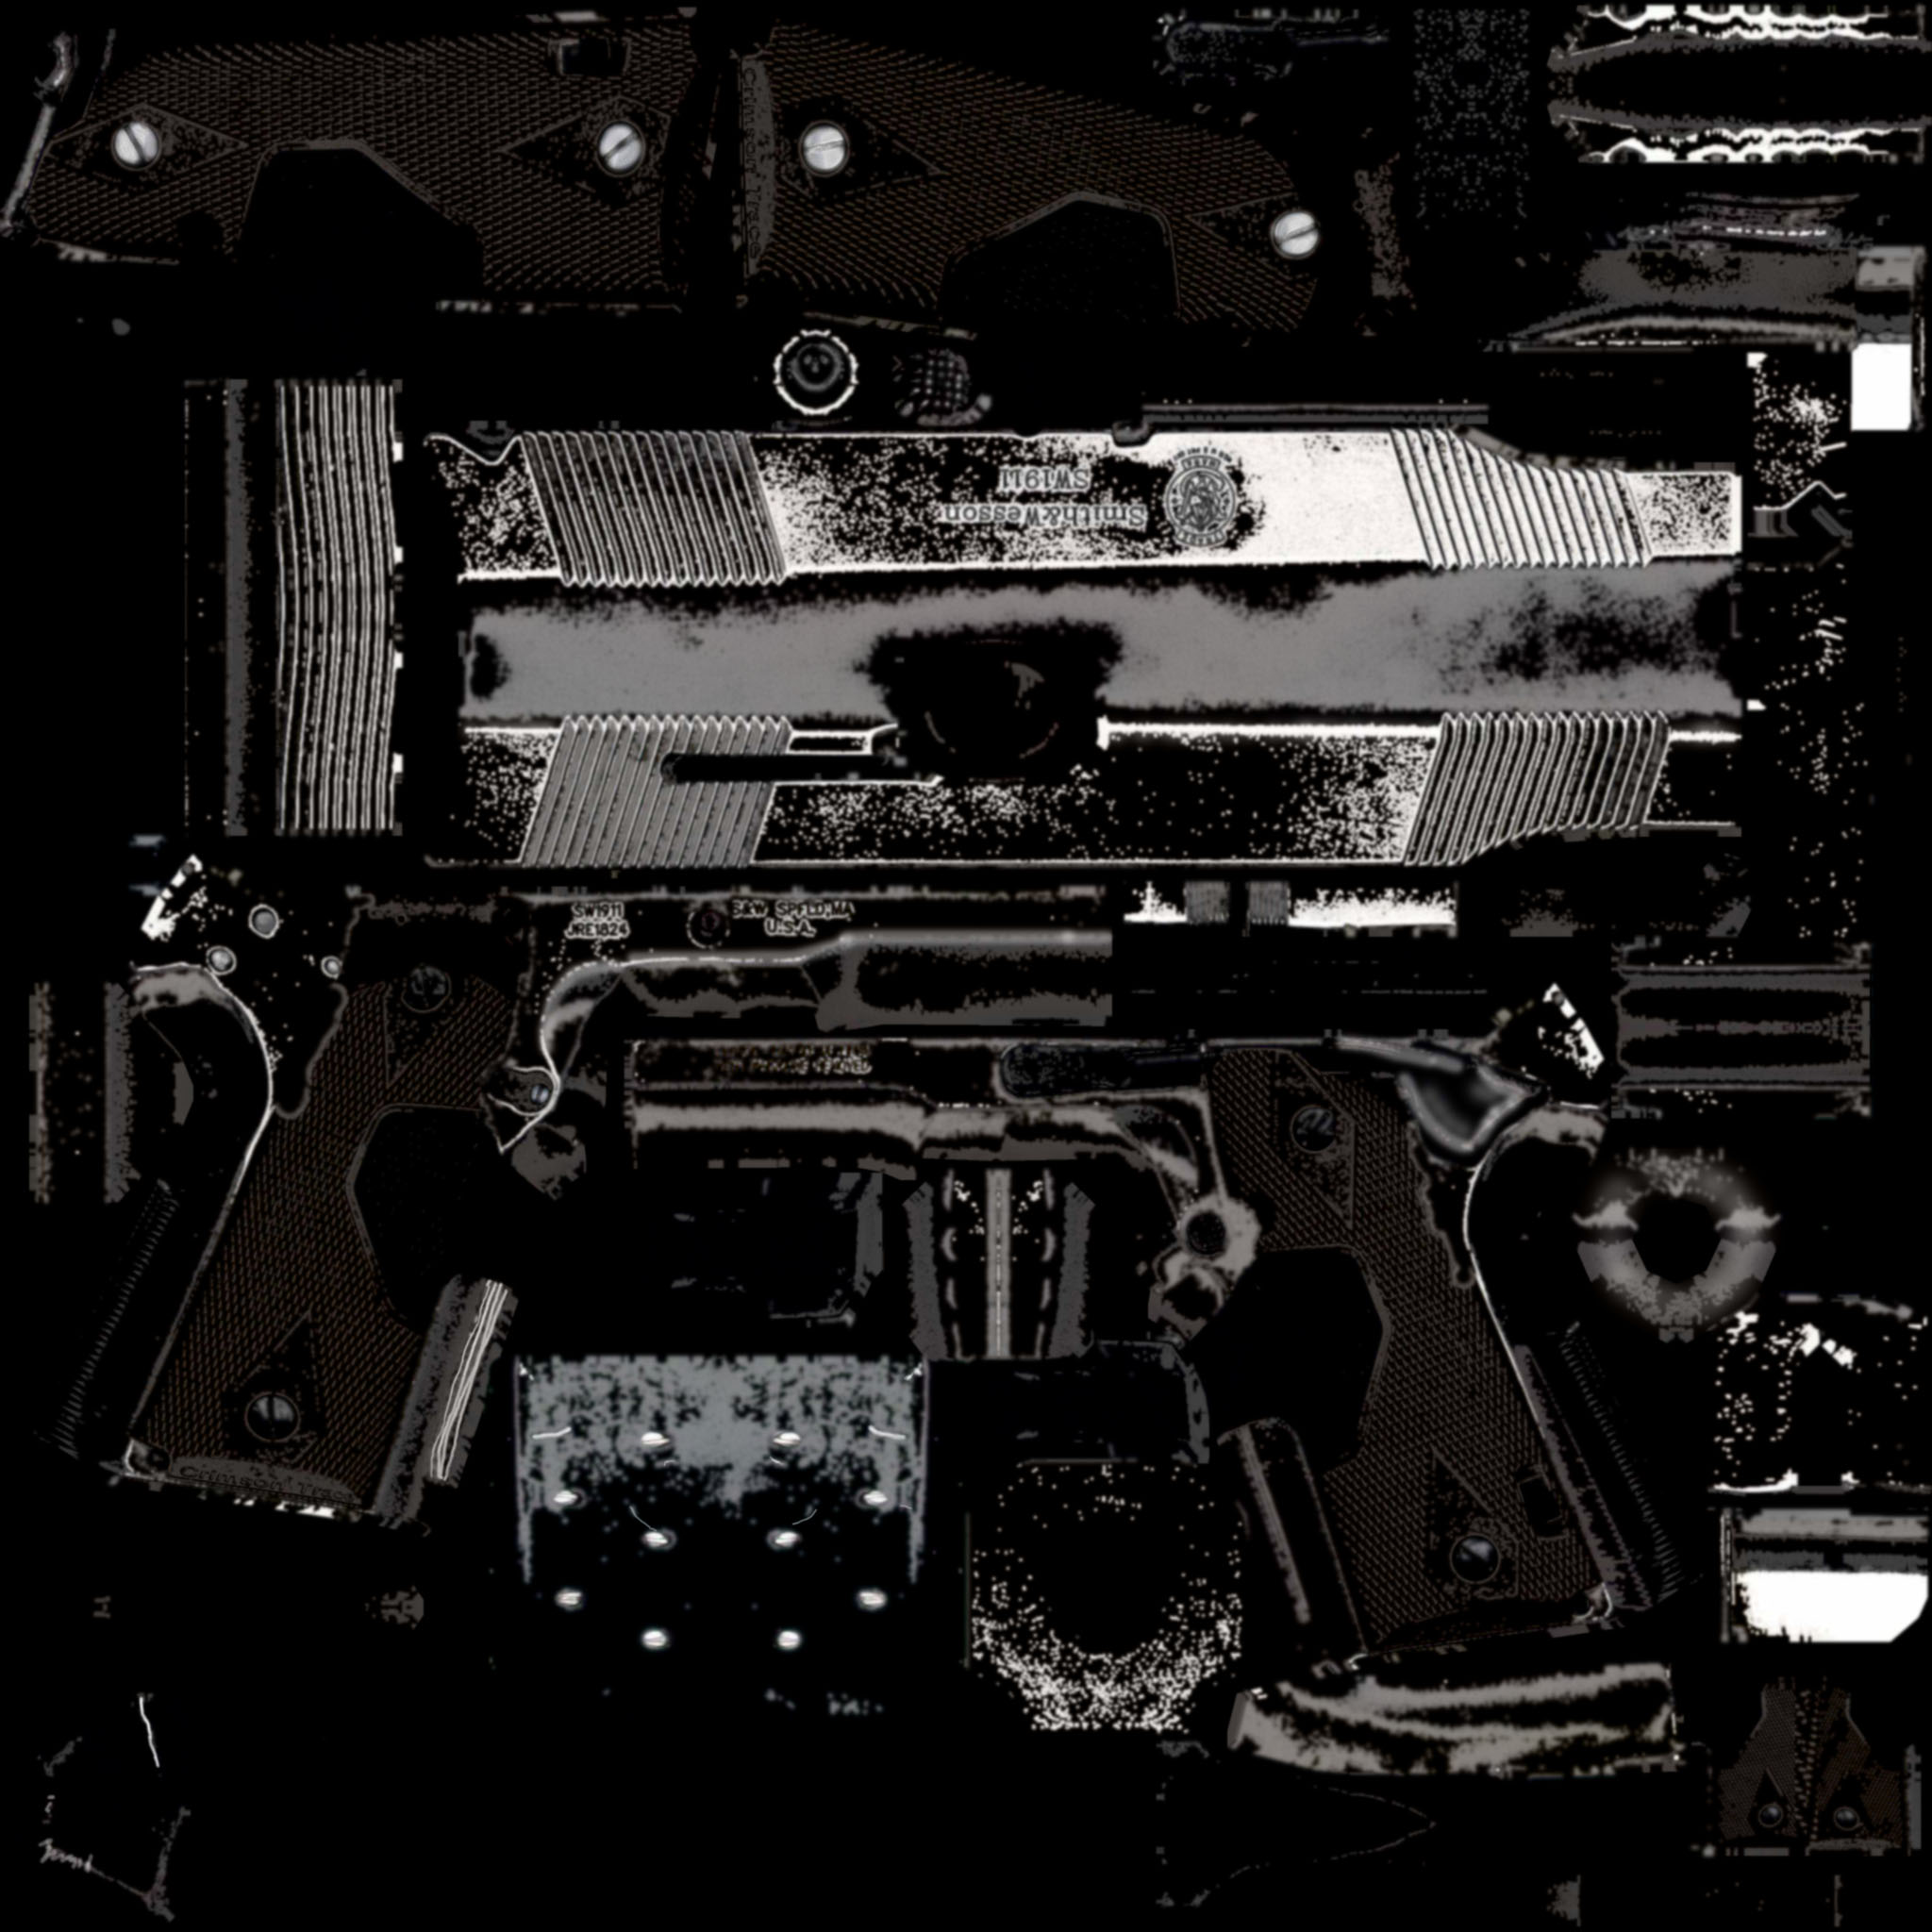
\includegraphics[width=9cm]{images/handgun-S.jpg}
    }
    \caption{\fontsize{11pt}{1.0cm}\zarbold\textbf{\lr{a gun specular map}}}
    \label{fig:my_label}
\end{figure}
      بعد از استفاده از این \lr{specular map} برای مدل اسلحه نتیجه به شکل زیر در می آید، می بینید که مقدار بازتاب در همه نقاط یکسان نیست:

\begin{figure}[H]
    \centering
    \href{https://github.com/devprofile98/shm}{
        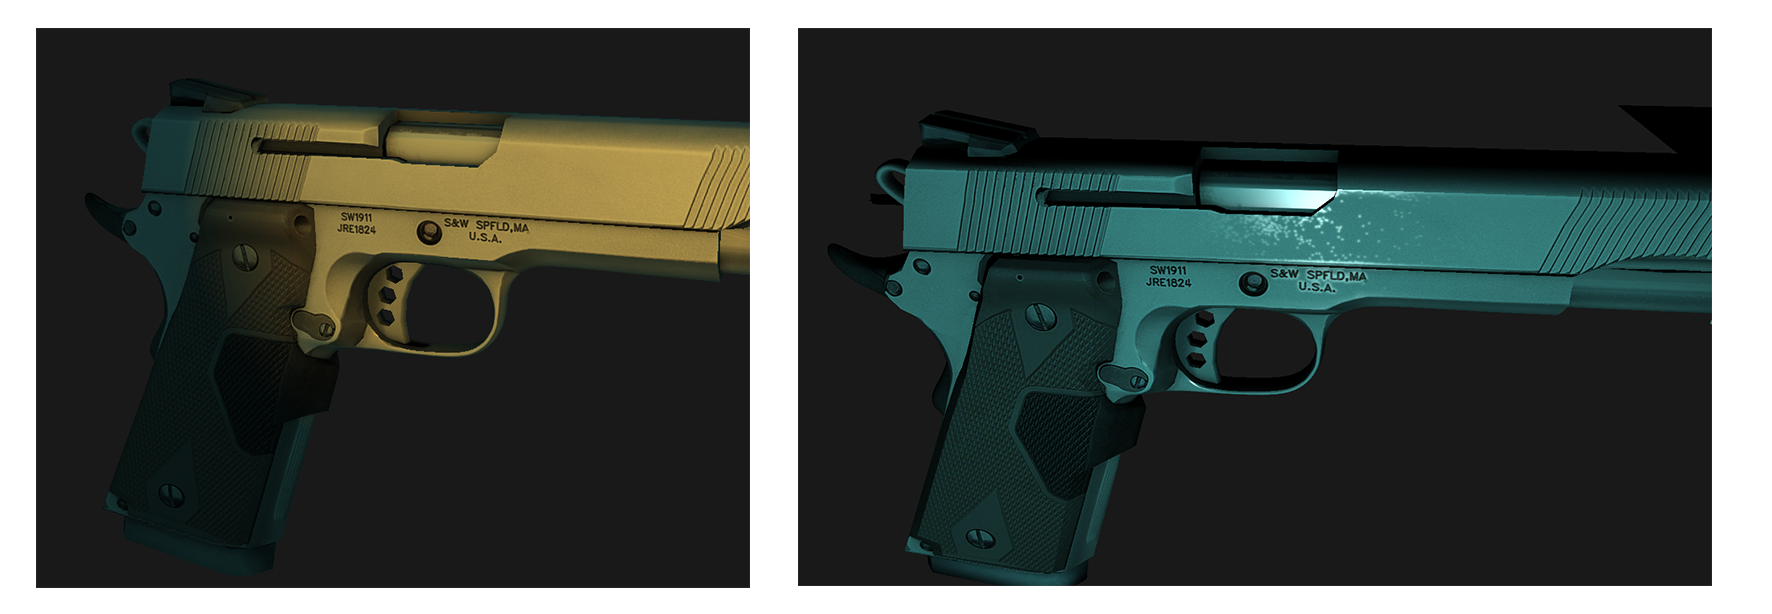
\includegraphics[width=15cm]{images/specular-gun.png}
    }
    \caption{\fontsize{11pt}{1.0cm}\zarbold\textbf{\lr{phong shaded gun}}}
    \label{fig:my_label}
\end{figure}

\newpage

\subsection{\lr{Shadows}}
    الگوریتم های زیادی برای تولید سایه وجود دارند، برخی از این الگوریتم ها مناسب \lr{real-time} نیستند و به همین دلیل مورد بحث ما نیستند، این الگوریتم ها غالبا از روش های \lr{ray-tracing} سرچشمه می گیرند، در الگوریتم های \lr{ray-tracing} به صورت خودکار سایه ها تولید می شوند، دلیل آن نیز نرسیدن پرتو های نور به نقاط است.\par
    روش هایی که برای تولید سایه در \lr{real-time} استفاده می کنیم شباهت زیادی از لحاظ تعریف به روش بالا دارند، باید سطوحی را پیدا کنیم که نور به آن ها نمی رسد، یکی از این روش ها \lr{shadow mapping} نام دارد، این روش و مشتقات آن در بازی کامپیوتری مورد استفاده قرار می گیرند. \lr{shadow mapping} روشی ساده است که در مراحلی که در زیر شرح می دهم قابل تولید است:\\ اساس کار ایجاد نقشه ای است که با استفاده از آن می توانیم مشخص کنیم که نور به چه جسمی زودتر برخورد کرده و چه جسمی به منبع نور نزدیک تر است.

\begin{figure}[H]
    \centering
    \href{https://github.com/devprofile98/shm}{
        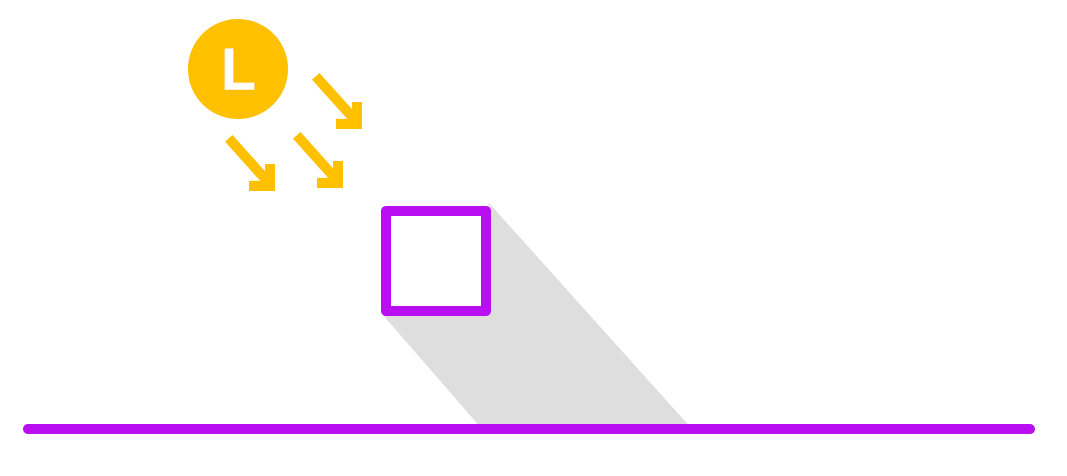
\includegraphics[width=11cm]{images/shadow.png}
    }
    \caption{\fontsize{11pt}{1.0cm}\zarbold\textbf{\lr{absence of light - shadow}}}
    \label{fig:my_label}
\end{figure}

    همانگونه که در شکل بالا نیز پیداست، سایه به دلیل نرسیدن نور و غیاب نور در نقطه پدید می آید، در روش \lr{shadow mapping} ابتدا صحنه را از دید منبع نور\footnote{\lr{Light View}} به صورت ساده رندر می کنیم، در این عملیات ما \lr{fragment shader} را خالی می گذاریم، زیرا نیازی به خروجی آن نداریم، تنها کاری که باید انجام شود پر شدن بافر عمق\footnote{\lr{Depth Buffer}} است، این کار به صورت خودکار انجام می شود پس ما نیازی به نوشتن کد در \lr{fragment shader} نداریم، \lr{depth buffer} تشکیل شده را به یک تکسچر متصل می کنیم، به این صورت \lr{shadow map} ما آماده است.\par
    بعد از اینکه \lr{shadow map} آماده شد، حالا صحنه را از اول و با تمام جزئیات موردنیاز رندر می کنیم، و در \lr{fragment shader} تصمیم می گیریم که آیا این نقطه نزدیک ترین نقطه در برخورد با پرتو نور است یا خیر، برای اینکار نیاز داریم که نقطه ای که در حال پردازش است را به \lr{light space} ببریم، این کار در مرحله \lr{vertex shader} و توسط \lr{light Space Matrix} انجام می شود، مقدار این ضرب به مرحله \lr{fragment shader} فرستاده می شود و به شکل زیر برای محاسبه نور استفاده می شود:

    \begin{LTR}
    \small
        \begin{lstlisting}[style=C++Style,caption=\lrit{calculate shadow}]
float ShadowCalculation(vec4 fragPosLightSpace)
{
    // perform perspective divide
    vec3 projCoords = fragPosLightSpace.xyz / fragPosLightSpace.w;
    // transform to [0,1] range
    projCoords = projCoords * 0.5 + 0.5;
    // get closest depth value from light's perspective (using [0,1] range fragPosLight as coords)
    float closestDepth = texture(shadowMap, projCoords.xy).r;
    // get depth of current fragment from light's perspective
    float currentDepth = projCoords.z;
    // check whether current frag pos is in shadow
    float shadow = currentDepth > closestDepth  ? 1.0 : 0.0;

    return shadow;
}
        \end{lstlisting}
    \end{LTR}
    \normalsize
    \vspace*{0.3cm}

     در تابع بالا ابتدا مقادیر
     $[x, y, z]$
     تقسیم بر مقدار
     $w$
     می شوند زیرا \lr{light space matrix} به صورت \lr{orthogonal} محاسبه شده بود، زیرا همانطور که پیش تر گفتیم پرتو های نور با یکدیگر موازی هستند و اگر بخواهیم از دید منبع نور جهان را رندر کنیم باید از نوع دیداری استفاده کنیم که \lr{orthogonal} باشد، حالا اما برای استفاده در رندر نهایی نیاز به \lr{perspective view} داریم، برای همین این تقسیم را انجام می دهیم. در مرحله بعد مقادیر را به بازه
     $[0-1]$
     می آوریم، از پیش میدانیم که مقادیر بین
     $[-1, 1]$
     هستند پس با تقسیم کردن به دو و جمع با $0.5$ به بازه دلخواه ما منتقل می شوند. در مرحله بعد مقدار \lr{closest depth} را از تکسچری که در مرحله قبل رندر کرده بودیم دریافت می کنیم، این مقدار، نزدیک ترین جسم به نور است، در خط بعد این مقدار را با عمق نقطه فعلی در نظر مقایسه می کنیم، اگر عمق فعلی از نزدیک ترین عمقی که داریم بیشتر باشد پس این پیکسل در سایه است پس مقدار 1.0 به معنی \lr{True} برمی گردانیم. حاصل کارهای بالا به ساختن سایه منجر می شود:

\begin{figure}[H]
    \centering
    \href{https://github.com/devprofile98/shm}{
        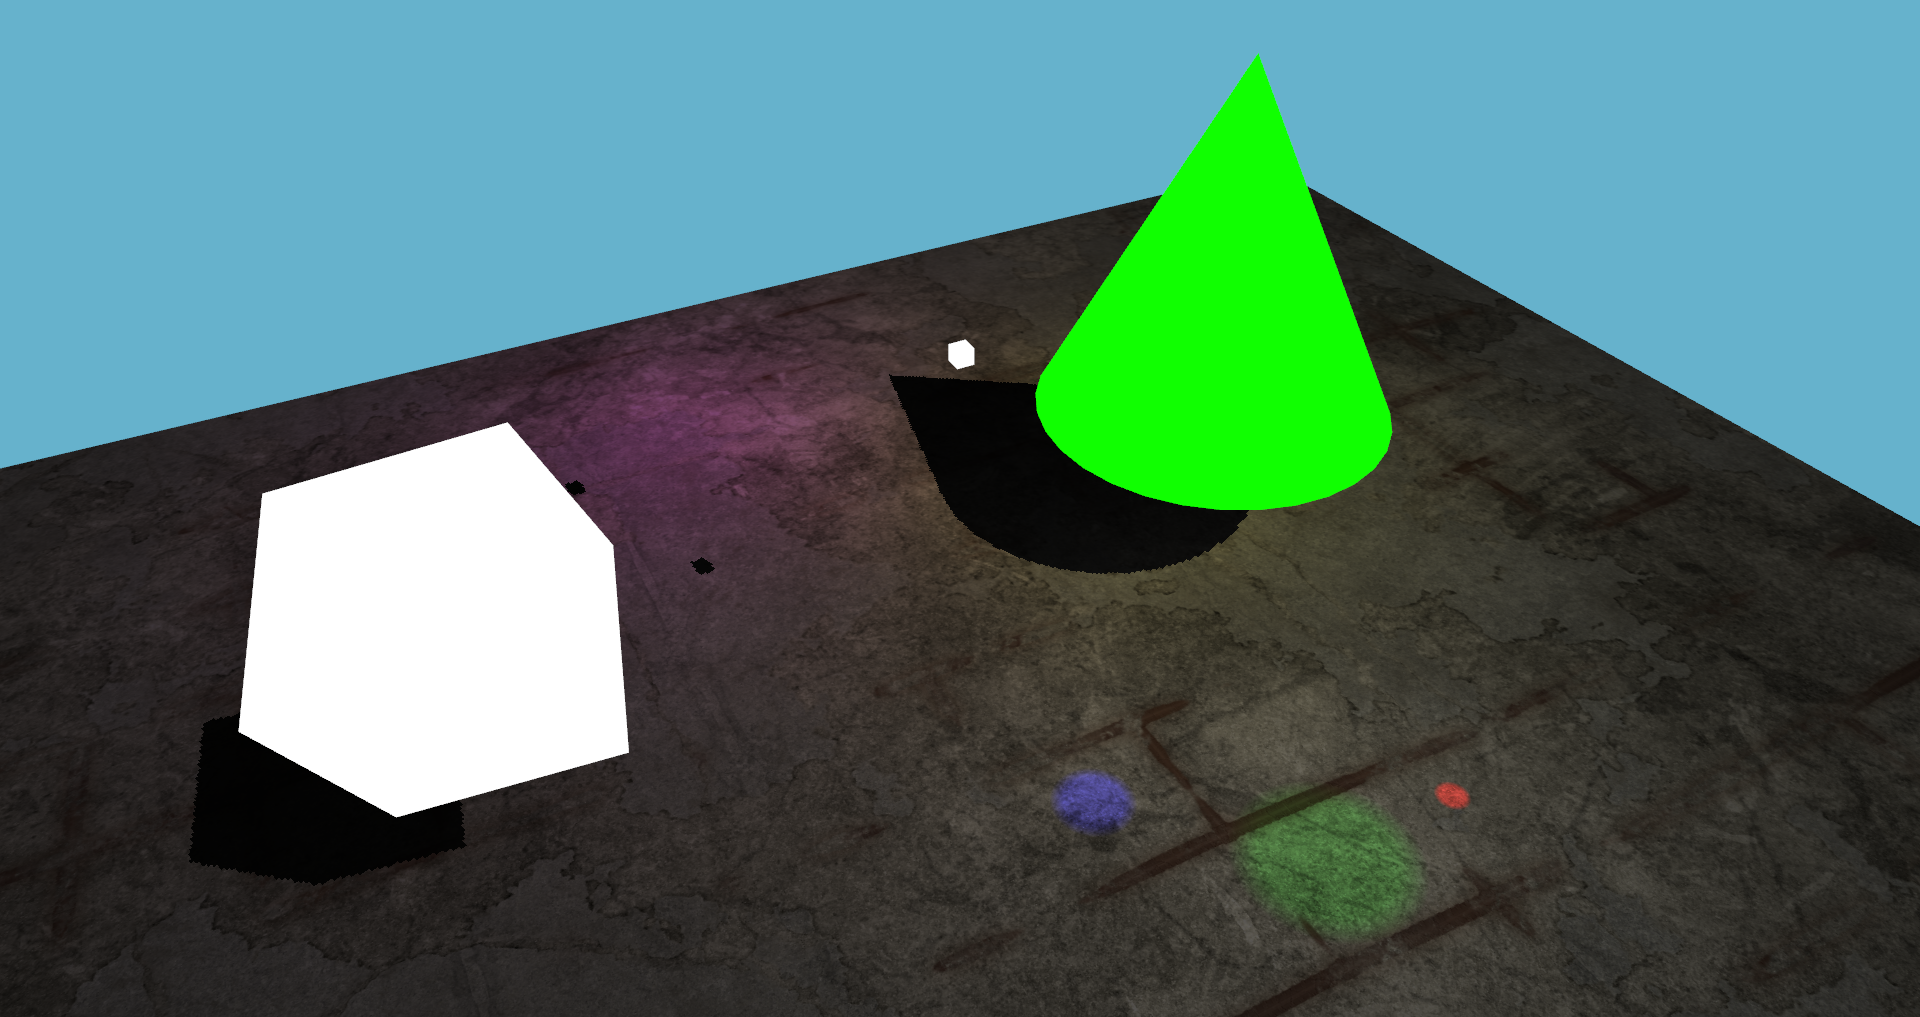
\includegraphics[width=13cm]{images/sceme-shadow.png}
    }
    \caption{\fontsize{11pt}{1.0cm}\zarbold\textbf{\lr{scene with shadow}}}
    \label{fig:my_label}
\end{figure}

\newpage
%\addcontentsline{toc}{section}{کاربردها}
\section{\fontsize{15pt}{1.0cm}\zarbold\textbf{جمع بندی و نتیجه گیری}}
\vspace*{0.6cm}
\noindent
\normalsize
    \subsection{نتیجه گیری}
    در دنیای امروز، صنایعی که بر پایه گرافیک کامپیوتر شکل گرفته اند سهم عظیمی از گردش مالی، کارآفرینی و ساعات کار و اوقات فراغت تعداد زیادی از مردم را تشکیل می دهند، در این بین شرکت ها و موسسات بزرگ با روی آوردن به موتور های رندر بی درنگ در پی افزایش بازدهی و کاهش هزینه های خود هستند. به دنبال افزایش قدرت کارت های گرافیک، واقع گرایی هر چه بیشتر همچنان فرصت را برای استفاده از موتور های رندر با دقت بسیار بالا در مصارف بی درنگ را از صنایع و کمپانی های بزرگ گرفته است.\par
    استفاده شرکت ها و نرم افزار های متن باز\footnote{\lr{Open Source}} سبب تمایل بیشتر کاربران به محصولات آن ها شده است. این مهم سبب علاقمندی هر چه بیشتر شرکت ها به موتور های رندر بلادرنگ با تکنولوژی های به روز تر شده است.
     برای مثال گوشه ای از کاربرد های این نرم افزار ها را در موتور \lr{Eevee} می بینیم. \lr{Eevee} موتور رندر سه بعدی \lr{realtime} استفاده شده در نرم افزار \lr{blender} است، \lr{Eevee} به منظور افزایش سرعت در زمان توسعه و گاها در محصولات تجاری عرضه شده است.
    در زمان کار با \lr{blender} و در صحنه های بزرگ و شلوغ با استفاده از \lr{Eevee} می توانیم با سرعت بالا دسترسی به اکثر جزئیات و ویژگی های صحنه خود داشته باشیم، اینکار بدون استفاده از  یک \lr{real time renderer} مانند \lr{Eevee} پروسه ای بسیار زمان بر و شامل آزمون و خطاهای زیادی می باشد که هزینه هایی زیادی از نظر مالی و نیروی انسانی به جای می گذارد، \lr{Eevee} به صورت ماژولار و منطبق با قرارداد های \lr{Blener} ساخته شده. همچنین  \lr{Eevee}  با استفاده از \lr{openGL} و تکنیک های \lr{render}  استفاده شده در صنعت بازی سازی موفقیت های زیادی کسب کرد.\par
    موتوری که در این پروژه توسعه دادم از لحاظ نرم افزاری در دسته بندی نرم افزار هایی مانند \lr{Eevee} قرار می گیرد، \lr{Shm} مانند \lr{Eevee} متمرکز بر تولید سریع و شبیه سازی مطابق با واقعیت\footnote{\lr{Photo realistic}} تصاویر است، اجزا زیادی مانند:
    \begin{persian}
    \begin{enumerate}
      \item ارائه دو مدل دوربین \lr{perspective}  و \lr{ortho}
      \item ارائه سه نوع کلی از \lr{light caster} مانند \lr{point}, \lr{directional or sun} و \lr{spot}
      \item تولید \lr{light effect} ها مانند \lr{highlight} و \lr{shadow}
      \item \lr{component} هایی برای کنترل تصاویر، \lr{textures} و \lr{gpu buffer} ها
      \item  کنترل خودکار و دستی \lr{uniform buffer objects}
      \item ارائه کلاس \lr{Model} برای \lr{load} کردن مدل های سه بعدی و مدیریت کردن \lr{material}, \lr{ambient and specular texture maps} و ویژگی های آن ها
      \item ارائه کلاس ها برای \lr{load} و \lr{compile} کردن \lr{shader} ها
      \item و کلاس های عمومی تر برای بیان کردن رنگ ها و ساختار های ریاضی مانند \lr{vector} های سه و چهار بعدی، \lr{Matrix} های سه در سه و چهار در چهار, \lr{Quaternion}
      \item ...
    \end{enumerate}
\end{persian}

    توسط \lr{shm} ارائه می شود.\par

    \newpage
    \subsection{مشاهده  گر سه بعدی}
    این پروژه قابل استفاده برای \lr{3D scene viewer} ها مانند \lr{Microsoft 3D viewer} است:
\begin{figure}[H]
    \centering
    \href{https://github.com/devprofile98/shm}{
        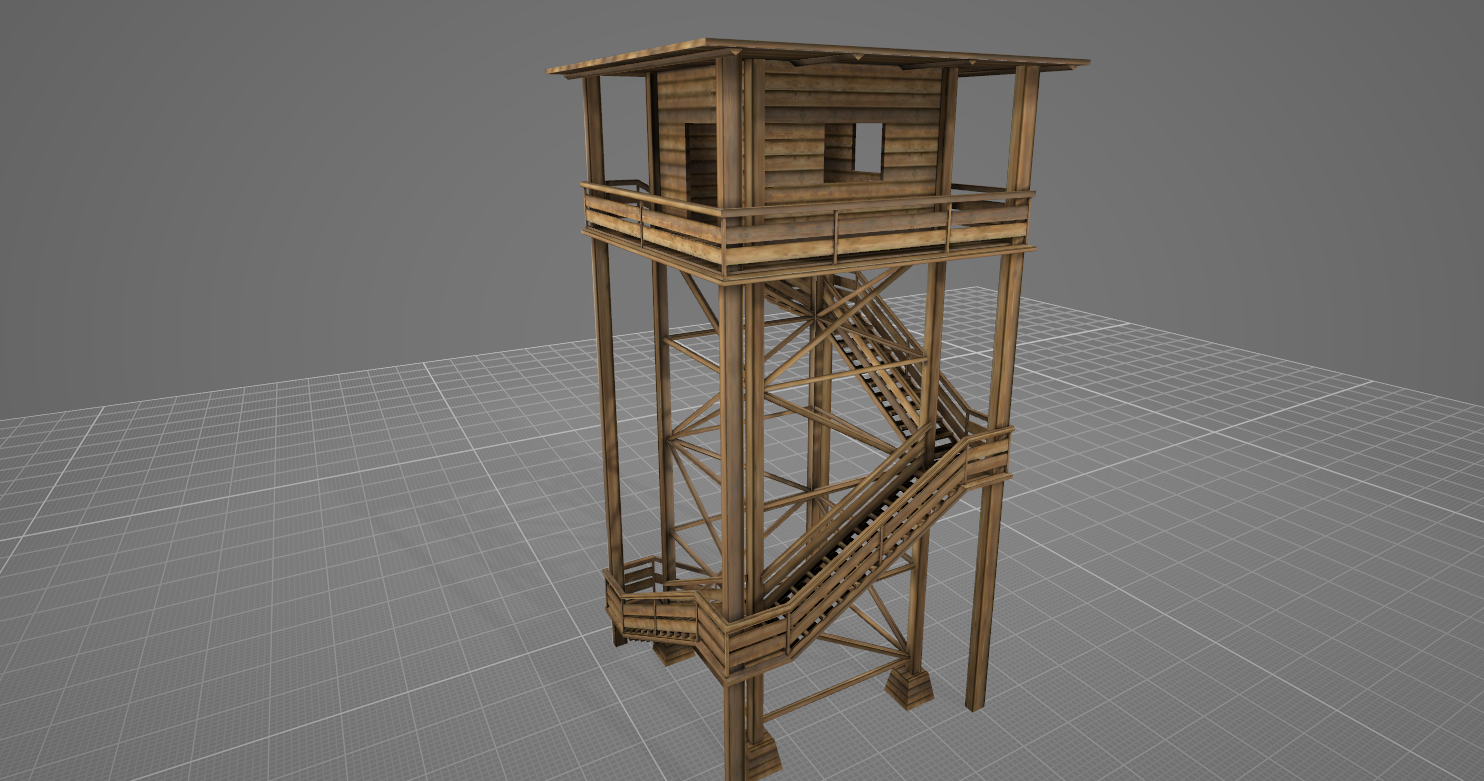
\includegraphics[width=13cm]{images/archerym3d.png}
    }
    \caption{\fontsize{11pt}{1.0cm}\zarbold\textbf{\lr{model in microsoft 3d viewer}}}
    \label{fig:my_label}
\end{figure}

\begin{figure}[H]
    \centering
    \href{https://github.com/devprofile98/shm}{
        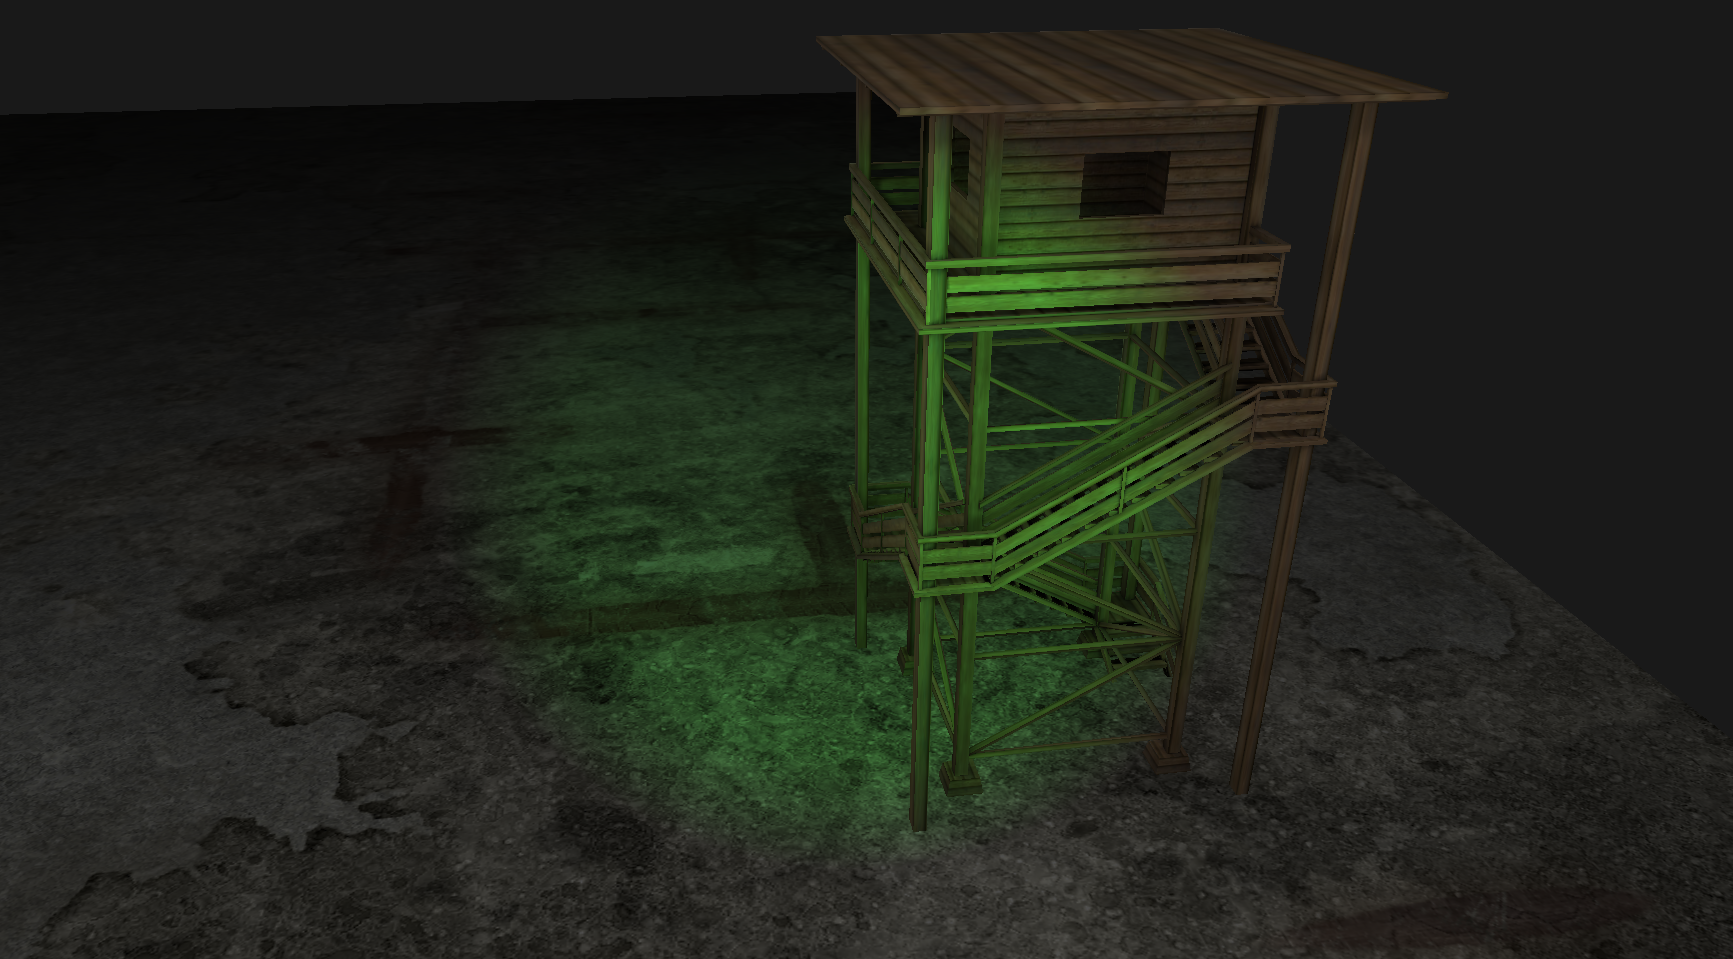
\includegraphics[width=13cm]{images/archerys3d.png}
    }
    \caption{\fontsize{11pt}{1.0cm}\zarbold\textbf{\lr{model in my project wit a green point light and ground}}}
    \label{fig:my_label}
\end{figure}

    \newpage
    \subsection{بازی های ویدیویی}
    یکی از کاربرد های \lr{real-time render engine} ها همانطور که گفته شد، در صنعت بازی سازی است، در ادامه بازی معروف \lr{Flappy bird} که یک بازی دو بعدی و \lr{Arcade} است را در با اشیاء سه بعدی بازسازی می کنیم، در این بازی باید با فشردن درست \lr{space} پرنده را از بین \lr{pipe} ها عبور دهیم:

\begin{figure}[H]
    \centering
    \href{https://flappybird.io/}{
        
\includegraphics[width=13cm]{images/op-flappybird.png}
    }
    \caption{\fontsize{11pt}{1.0cm}\zarbold\textbf{\lr{original flappy bird}}}
    \label{fig:my_label}
\end{figure}

    برای شروع ابتدا مدل های \lr{pipe} و  \lr{bird} را در \lr{blender} می سازیم، سپس یک فایل جدید ایجاد می کنیم و \lr{shm} را به وسیله کد زیر به آن اضافه می کنیم:

        \begin{LTR}
    \small
        \begin{lstlisting}[style=C++Style,caption=\lrit{adding Engine to project}]
#include "Engine.hpp" // include needed component and classes for rendering
#include "Light.hpp" // if you want light caster in scene, include them
        \end{lstlisting}
    \end{LTR}
    \normalsize
    \vspace*{0.3cm}
\newpage

    دو \lr{shader} متفاوت برای پرنده و لوله ها می سازیم:
\begin{LTR}
    \small
        \begin{lstlisting}[style=C++Style,caption=\lrit{creating shaders}]
std::shared_ptr<shader> pipeshader = Engine::CreateShader("./assets/shaders/model_loading.vs", "./assets/shaders/model_loading.fs");
std::shared_ptr<shader> birdshader = Engine::CreateShader("./assets/shaders/model_loading.vs", "./assets/shaders/model_loading.fs");
        \end{lstlisting}
    \end{LTR}
    \normalsize
    \vspace*{0.3cm}
    همچنین قابلیت استفاده از یک \lr{shader} برای هر دو شی در بازی وجود دارد.\par
    دو تابع ویژه حتما باید در این فایل تعریف شوند، تابع های \lr{inLoop} و \lr{outLoop} را در همین فایل تعریف می کنیم، وظیفه این تابع ها از نام آن ها پیداست، تابع \lr{inLoop} در \lr{main render loop} بازی صدا زده می شود، پس ویژگی های متغیر و مورد نیاز که در هر \lr{frame} باید اجرا شوند را در این تابع می نویسیم، کار تابع \lr{outLoop} این است که تنظیمات و اعمالی که قبل از شروع \lr{render loop} انجام می شود را انجام دهد، برای مثال ما فقط یکبار نیاز به \lr{load} کردن مدل ها در بازی داریم و آن هم قبل از اجرای \lr{render loop} است، پس به شکل زیر مدل هارا در بازی \lr{load} می کنیم.

\begin{LTR}
    \small
        \begin{lstlisting}[style=C++Style,caption=\lrit{loading a 3D model}]
Engine::getRenderer()
            ->LoadModel(
                "./assets/models/texturedbird.obj", // path to 3D model
                birdshader
                );
        \end{lstlisting}
    \end{LTR}
    \normalsize
    \vspace*{0.3cm}

    با استفاده از توابع موجود در \lr{Model} می توانیم \lr{position}, \lr{rotation} و  \lr{scale} مدل را تغییر دهیم، اینکار را برای مدل \lr{bird} به شکل زیر انجام می دهیم تا در موقعیت شروع بازی قرار بگیرد:

    \begin{LTR}
    \small
        \begin{lstlisting}[style=C++Style,caption=\lrit{position, scale, rotation}]
    GET_MODEL(bird)->setPosition({-3.0f, 5.7f , 0.0f});
    GET_MODEL(bird)->setScale({0.5f, 0.5f, 0.5f});
    GET_MODEL(bird)->setRotation({0.0f, 1.0f, 0.0f}, 45.0f);
        \end{lstlisting}
    \end{LTR}
    \normalsize
    \vspace*{0.3cm}

    مدل مربوط به \lr{pipe} را به شکل بالا \lr{load} می کنیم، چون \lr{pipe} به تعداد زیادی در محیط بازی قرار دارد، آن را با استفاده از دستور\lr{DrawInstances} در تابع \lr{inLoop} در محیط بازی رسم می کنیم:
        \begin{LTR}
    \small
        \begin{lstlisting}[style=C++Style,caption=\lrit{draw instances of a model}]
GET_MODEL(0)->DrawInstances(pipes_pos, nullptr);
        \end{lstlisting}
    \end{LTR}
    \normalsize
    \vspace*{0.3cm}
    در تابع بالا، آرگومان اول آرایه ای از \lr{glm::vec3} است که بیانگر مشخصات قرار گیری هر کدام از \lr{pipe} ها است، این مقادیر در تابع \lr{outLoop} به وسیله یک حلقه تولید شده اند.\par
    برای بررسی برخورد \lr{bird} و \lr{pipe} ها در بازی از تابع زیر استفاده می کنیم، اگر پرنده با یکی از لوله ها برخورد کند به حالت \lr{sleep} تغییر وضعیت می دهد و فیزیک بازی تاثیری بر آن ندارد، از این حالت برای \lr{reset} کردن بازی استفاده می کنیم.
    تصویری از محیط در حال اجرای بازی به شکل زیر است:
    \begin{figure}[H]
    \centering
    \href{https://github.com/devprofile98/shm}{
        
\includegraphics[width=14cm]{images/flappybird.png}
    }
    \caption{\fontsize{11pt}{1.0cm}\zarbold\textbf{\lr{my project flappy bird}}}
    \label{fig:my_label}
\end{figure}
    برای دانلود بازی می توانید از این \href{https://github.com/devprofile98/shm/releases/tag/v0.1-alpha}{لینک} استفاده کنید، همچنین برای دیدن فیلم اجرای بازی می توانید از این \href{https://youtu.be/JqjluAjQV84}{لینک} استفاده کنید.

\end{document} 